\documentclass[]{settings/wi-thesis}
\addbibresource{library.bib}

\begin{document}
\titleThesis{Prédiction du temps de cuisson de haricots basée sur TinyML en utilisant des données de temps de cuisson et des images de haricots}

\author{MBAIGOLMEM DANG-DANG THIERY}

% % Matriculation Number
% \id{20A179FS}

% % Field of Study
% \field{Ing\'enerie Informatique}

% % Address, for declarations at the end of the thesis.
% \city{Université de Ngaoundéré}

% \professor{Prof. Dr. Ing. FENDJI JEAN LOUIS KEDIENG EBONGUE}

% \supervisor{Supervisor, Pr Dr BOUKAR}

% Submission Date
% \date{08.09.2025}
\begin{titlepage}
	\begin{tikzpicture}[remember picture,overlay]
		\tikzset{
			trait/.style={draw=blue!70!white,rounded corners,align=center,double,line width=7pt}}
		\tikzset{
			them/.style={draw=blue!70!black,line width=4pt,rounded corners,text justified, text width=0.75\linewidth,fill=white}}
		\draw[trait,top color=green!80!cyan,bottom color=green!80!cyan](current page.north west) -- (current page.north east)--(current page.south east)--(current page.south west)--cycle;
		
		\node[yshift=-2cm,xshift=0.5cm](univ) at (current page.115){\normalsize{} \bfseries UNIVERSITE DE NGAOUNDERE};
		\node[yshift=-2cm,xshift=5cm](univ) at (current page.110){\includegraphics[width=0.1\linewidth,height=1.5cm]{logou.png}};
		\node[yshift=-3cm,xshift=0.5cm](fac) at (current page.115){\normalsize{} \bfseries FACULTE DES SCIENCES};
		\node[yshift=-3.6cm,xshift=5cm](univ) at (current page.110){\includegraphics[width=0.05\linewidth,height=1cm]{logo.png}};
		\node[yshift=-4cm,align=center](dep) at (current page.115){\hspace*{1cm}\normalsize{} \textbf{ Département de Mathématiques  }};
		\node[yshift=-5cm,align=center](dep) at (current page.115){\hspace*{1cm}\normalsize{} \textbf{et Informatique }};
		
		\node[yshift=-2cm,xshift=11cm](univa) at (current page.110){\normalsize{} \bfseries THE UNIVERSITY OF NGAOUNDERE};
		\node[yshift=-3cm,xshift=11cm](faca) at (current page.110){\normalsize{} \bfseries FACULTY OF SCIENCE};
		\node[yshift=-4cm,align=center,xshift=10.5cm](depa) at (current page.110){\hspace*{1cm}\normalsize{} \textbf{ Department of Mathematics }};
		\node[yshift=-5cm,align=center,xshift=10.5cm](depa) at (current page.110){\hspace*{1cm}\normalsize{} \textbf{ and Computer Science }};
		
		
		\node[yshift=-10cm,xshift=5cm,align=center](mem) at (current page.110){\bfseries{}\large{} Mémoire de Master Recherche};
		\node[yshift=-11cm,xshift=5cm,align=center](pres) at (current page.110){{\bfseries Présenté en vue de l'obtention du dipl\^ome de Master}};
		\node[yshift=-12cm,xshift=5cm,align=center](ment) at (current page.110){{\bfseries  en Ingénierie Mathématiques}};
		\node[yshift=-13.2cm,xshift=5cm,align=center](ment) at (current page.110){{\bfseries  Option: Probabilité et Statistique}};
		\node[yshift=-14.2cm,xshift=5cm,align=center](tith) at (current page.110){{\bfseries  THEME:}}; 
		\node[them,yshift=-16cm,xshift=6cm](them) at (current page.110){{\bfseries \Large{} Techniques d'échantillonnage et enqu\^ete par sondage sur le choix des étudiantes vers les filières scientifiques ou technologiques:  cas de l'Université de Ngaoundéré, année académqiue $\mathbf{2023/2024}$ }}; 
		\node[yshift=-19cm,xshift=5cm](redac) at (current page.110){{\bfseries Rédigé par: MBELAWADZAI Joseph }};
		\node[yshift=-19.8cm,xshift=3.88cm](matr) at (current page.110){{\bfseries Matricule: $\mathbf{17A292FS}$ }};
		
		\node[yshift=-21cm,xshift=3.88cm](imp) at (current page.110){{\bfseries Sous l'encadrement de: }};
		\node[yshift=-21.8cm,xshift=5cm](imp) at (current page.110){{\bfseries Dr MBOUNJA BESSEME FRITZ  }};
		\node[yshift=-24.8cm,xshift=5cm](imp) at (current page.110){{ \shadowbox{\color{cyan!85!red}\bfseries \textcolor{black}{Septembre 2024}} }}; 
	\end{tikzpicture}
\end{titlepage}
\maketitle

\chapter*{DEDICACE}\addcontentsline{toc}{chapter}{Dédicace}
\vspace*{7cm}
\begin{cursive}
	{\Huge Je dédie ce travail à ma famille avec tous mes sentiments de respect, d'amour, de gratitude et de
		reconnaissance.}
\end{cursive}
\chapter*{REMERCIEMENTS}\addcontentsline{toc}{chapter}{Remerciements}
La production de ce mémoire a nécessité beaucoup d’énergies et du temps. J’aimerais remercier ici tous ceux qui de près ou de loin ont contribué et ont donné de leur temps pour que mon étude soit menée à bien. Tout d'abord je rends gr\^ace au Seigneur Dieu Tout Puissant qui m'accorde tous les jours non seulement le souffle de vie, mais l'intelligence et la sagesse pour accomplir des \oe uvres au quotidien. \\
Nos remerciements  vont aussi précisément à l'endroit du:
\begin{itemize}
	\item  Recteur de l'Université de Ngaoundéré,  {\footnotesize\bfseries Pr MAMOUDOU Abdoulmoumini} , qui a rendu possible notre étude en Master 2;
	\item  Doyen de la Faculté des Sciences de l'Université de Ngaoundéré, {\footnotesize\bfseries Pr DJONKA Dieudonné}, pour avoir organisé nos études tout en préservant la discipline;
	\item Chef de département de Mathématiques et Informatique,  { \footnotesize\bfseries Pr.Dr.Ing. DAYANG Paul}, pour l'accompagnement et l'orientation donnée à notre travail;
	\item Directeur de ce mémoire,  {\footnotesize\bfseries Pr Dr Ing. FENDJI JEAN LOUIS KEDIENG EBONGUE}, qui nous a accompagnés et encadrés pendant tout le temps de rédaction et a su nous guider à travers des recommandations pour la réalisation de cette étude;
\end{itemize}
\par Ensuite, nous exprimons notre gratitude à tous les enseignants du département de mathématiques et informatique, pour
les différents cours dispensés depuis le cycle licence, pour les orientations nécessaires à notre travail et pour la disponibilité dont ils ont fait preuve lorsque nous nous sommes référés à eux.
\par Enfin, nos gratitudes vont à l'endroit des parents, collègues et camarades, pour les différents moyens et aides nécessaires qu'ils nous ont été apportés. Je citerai:
\begin{itemize}
	\item  Mes parents, pour tout ce que vous faites dans ma vie;
	\item {\footnotesize \bfseries Ousmane H., A. LeBon, Ibrahim A., Layibe P. }, mes camardes de promotion, pour la collaboration et la discussion tout au long de ce travail. Vous êtes les meilleurs !;
	\item   Mes frères et s\oe urs pour leurs convivialités et encouragements.
\end{itemize}



\input{content/00-Abstract.tex}
\chapter*{Résumé}

L’optimisation des procédés de transformation agroalimentaire est un enjeu majeur pour améliorer la qualité, réduire les coûts et limiter le gaspillage. Dans ce contexte, la cuisson des haricots occupe une place centrale, leur temps de cuisson influençant directement la texture, la valeur nutritionnelle et l’acceptabilité du produit. Les méthodes traditionnelles d’estimation, bien que précises, sont chronophages, destructives et peu adaptées à un contrôle en ligne. Ce mémoire explore l’apport du Tiny Machine Learning (TinyML) comme solution innovante pour prédire, à partir d’images, le temps de cuisson des haricots de manière non destructive et adaptée aux environnements contraints. La méthodologie adoptée repose sur un pipeline hybride combinant classification et régression. Après la constitution de jeux de données spécifiques, plusieurs architectures de réseaux de neurones légers (CNN personnalisés, MobileNetV2, EfficientNet-B0, NASNetMobile) ont été évaluées et optimisées par quantification pour un déploiement embarqué. Les résultats obtenus montrent que le modèle CNN conçu sur mesure atteint un compromis satisfaisant entre précision, latence et consommation mémoire. Intégré dans une application Android, le système démontre la faisabilité d’une prédiction embarquée fiable et rapide du temps de cuisson. Au-delà de la contribution technique, ce travail illustre le potentiel du TinyML dans l’agroalimentaire et ouvre des perspectives pour le développement d’outils intelligents, accessibles et économes en énergie, favorisant un contrôle qualité amélioré et durable.

\vspace{0.5cm}
\noindent\textbf{Keywords:} TinyML, vision par ordinateur, réseaux de neurones légers, haricots, temps de cuisson.

\tableofcontents
\listoffigures
\listoftables
\chapter*{Liste des abréviations}
\addcontentsline{toc}{chapter}{Liste des abréviations}

\begin{longtable}{|p{3cm}|p{11cm}|}
\hline
\textbf{Abréviation} & \textbf{Définition} \\
\hline
CNN & Convolutional Neural Network (réseau de neurones convolutifs) \\
\hline
FPU & Floating Point Unit (une unité du CPU qui effectue des calculs sur des nombres à virgule flottante) \\
MAE & Mean Absolute Error (erreur absolue moyenne), mesure de l’écart moyen entre les valeurs prédites et observées. \\
\hline

MAPE & Mean Absolute Percentage Error (erreur absolue moyenne en pourcentage) \\
\hline

MaxErr & Maximum Error (erreur maximale observée) \\
\hline

NASNetMobile & Neural Architecture Search Network Mobile \\
\hline

$R^2$ & Coefficient de détermination, mesure de la proportion de variance expliquée par le modèle. \\
\hline

RMSE & Root Mean Square Error (racine de l’erreur quadratique moyenne), mesure de l’écart quadratique entre prédictions et observations \\
\hline

TBNet & \textit{Tiny Bean (cooking time) Network}, architecture proposée pour la prédiction du temps de cuisson des haricots à partir d’images. 
Le suffixe \textbf{2} (TBNet2) correspond à une couche finale de 256 filtres, tandis que le suffixe \textbf{5} (TBNet5) correspond à 512 filtres \\
\hline

TinyML & Tiny Machine Learning, déploiement de modèles d’apprentissage automatique sur des dispositifs embarqués à faibles ressources \\
\hline

XAI & Explainable Artificial Intelligence (intelligence artificielle explicable), ensemble de méthodes visant à interpréter les décisions des modèles. \\
\hline
\end{longtable}


\chapter{Introduction g\'en\'erale}
\addcontentsline{toc}{chapter}{Introduction g\'en\'erale}

\section{Contexte et justification}
L’optimisation des procédés de transformation agroalimentaire est un enjeu stratégique pour améliorer la qualité des produits, réduire les coûts de production et limiter le gaspillage alimentaire. Parmi ces procédés, la cuisson des légumineuses, et notamment des haricots, occupe une place importante en raison de leur valeur nutritive, de leur consommation mondiale et de leur rôle dans la sécurité alimentaire \citep{mendoza2018}. Le temps de cuisson influence directement la texture, la saveur, la valeur nutritionnelle ainsi que l’acceptabilité du produit par le consommateur \citep{mbofung2012}.

Traditionnellement, l’estimation de ce temps repose sur des méthodes empiriques ou destructives, telles que la cuisson test ou la mesure de l’absorption d’eau. Bien que fiables, ces approches sont souvent coûteuses, longues et peu adaptées à un contrôle en temps réel. L’évolution récente de l’intelligence artificielle (IA) et des technologies embarquées offre de nouvelles perspectives pour automatiser et améliorer cette prédiction de manière non destructive.

Le \textit{Tiny Machine Learning} (TinyML), qui consiste à déployer des modèles d’apprentissage automatique sur des dispositifs embarqués à faible consommation énergétique et ressources limitées, se présente comme une solution prometteuse. Grâce à des architectures légères comme \textit{MobileNetV2} ou des réseaux de neurones convolutionnels compacts, il est désormais possible de traiter des données visuelles directement sur des microcontrôleurs ou des smartphones, ouvrant la voie à des systèmes intelligents accessibles même dans des environnements à faibles ressources \citep{banbury2021}.

Dans le domaine agricole, l’intégration de la vision par ordinateur et du TinyML a déjà démontré son efficacité pour l’estimation de la maturité des fruits, la détection de maladies et le suivi de la qualité des denrées périssables \citep{abdalla2023, tastan2023}. Ces avancées technologiques laissent entrevoir la possibilité d’estimer le temps de cuisson des haricots à partir d’images, de manière rapide et fiable, même sans connexion internet.

\section{Problématique}
Malgré les progrès réalisés dans la transformation agroalimentaire, la prédiction précise et non destructive du temps de cuisson des légumineuses reste un défi technique. Les approches traditionnelles présentent plusieurs limites :
\begin{itemize}
	\item \textbf{Temps et coût} : les méthodes classiques sont chronophages et peu adaptées à un contrôle en ligne.
	\item \textbf{Manque de portabilité} : la plupart des systèmes automatisés existants nécessitent des équipements coûteux ou encombrants.
	\item \textbf{Contraintes énergétiques et matérielles} : dans les zones rurales ou les petites unités de production, l’accès à une puissance de calcul élevée est limité.
\end{itemize}

La question centrale de ce mémoire peut ainsi se formuler comme suit :
\begin{quote}
	\textit{Comment concevoir et déployer un système de prédiction du temps de cuisson des haricots, basé sur l’analyse d’images, qui soit à la fois précis, portable et compatible avec les contraintes matérielles du TinyML ?}
\end{quote}

\section{Objectifs et contributions}

\subsection{Objectif général}
Développer et déployer un modèle TinyML capable de prédire le temps de cuisson des haricots à partir d’images, de manière non destructive et en temps quasi réel.

\subsection{Objectifs spécifiques}
\begin{enumerate}
	\item Constituer et prétraiter un jeu de données d’images de haricots avec annotation du temps de cuisson.
	\item Concevoir, entraîner et optimiser des modèles légers adaptés au déploiement embarqué (CNN compacts, MobileNetV2, EfficientNet-lite, etc.).
	\item Évaluer les performances des modèles en termes de précision, consommation mémoire et temps d’inférence.
	\item Intégrer et tester le modèle final sur une plateforme embarquée (microcontrôleur ou smartphone).
\end{enumerate}

\subsection{Contributions attendues}
\begin{itemize}
	\item Une méthodologie reproductible pour la prédiction visuelle du temps de cuisson des légumineuses.
	\item Un modèle optimisé, compatible avec les contraintes du TinyML.
	\item Une démonstration fonctionnelle sur un dispositif embarqué.
\end{itemize}

\section{Portée et limites de l’étude}
Cette recherche se concentre sur la prédiction du temps de cuisson des haricots secs, en utilisant uniquement des images RGB comme données d’entrée. Le jeu de données est constitué de plusieurs variétés de haricots, collectées dans des conditions contrôlées.

Les limites incluent :
\begin{itemize}
	\item La restriction aux données visuelles (sans capteurs hyperspectraux ou thermiques).
	\item L’évaluation sur un nombre limité de dispositifs embarqués.
	\item La dépendance à un jeu de données spécifique, pouvant limiter la généralisation à d’autres contextes.
\end{itemize}

\section{Organisation du mémoire}
Le présent mémoire est structuré de manière à guider progressivement le lecteur depuis le contexte général de l’étude jusqu’aux conclusions et perspectives. Il se compose des parties suivantes :

\begin{itemize}
	\item \textbf{Abstract} : une synthèse concise présentant le sujet, la méthodologie adoptée, les principaux résultats et les apports de ce travail.
	\item \textbf{Chapitre 1 - Introduction générale} : un exposé du contexte scientifique et applicatif, de la problématique étudiée, des objectifs poursuivis ainsi que des contributions attendues.
	\item \textbf{Chapitre 2 - Revue de la littérature} : une analyse critique des travaux existants relatifs à la prédiction du temps de cuisson des aliments, au TinyML et aux approches de vision par ordinateur appliquées au domaine agroalimentaire.
	\item \textbf{Chapitre 3 — Méthodologie et conception} : présentation de la démarche méthodologique, du protocole expérimental et de la conception du système proposé.
	\item \textbf{Chapitre 4 — Implémentation et déploiement} : description des choix technologiques, de l’implémentation logicielle et du processus de déploiement sur plateformes embarquées.
	\item \textbf{Chapitre 5 — Résultats et discussion} : analyse et interprétation des résultats obtenus, mise en perspective avec les travaux de la littérature et discussion des limites.
	\item \textbf{Chapitre 6 — Conclusion et perspectives} : synthèse des contributions majeures du mémoire et identification de pistes de recherche futures.
\end{itemize}
 
\chapter{Revue de la littérature}
\label{chap:revue_litterature}

\section{Introduction}
La revue de littérature a pour objectif de positionner le présent travail dans le paysage scientifique actuel en identifiant les contributions majeures, les lacunes existantes et les perspectives d’amélioration. Dans le cadre de ce mémoire, l’accent est mis sur deux axes complémentaires : (i) les recherches liées à la prédiction du temps de cuisson des légumineuses et aux travaux connexes dans le domaine de l’alimentation, et (ii) l’émergence du \textit{Tiny Machine Learning} (TinyML) comme solution pour le traitement embarqué de données sous des contraintes strictes de mémoire et d’énergie. L’articulation de ces deux domaines ouvre la voie à des applications innovantes dans le secteur agroalimentaire, en particulier pour la cuisson et la qualité des aliments.

\section{Intelligence artificielle et secteur agroalimentaire}
L’intelligence artificielle (IA) a profondément transformé le secteur agroalimentaire en introduisant des outils pour l’automatisation, la classification et l’optimisation des procédés \cite{kamilaris2018}. La vision par ordinateur, notamment, est devenue un outil incontournable pour analyser l’apparence des fruits et légumes, estimer leur maturité, évaluer leur qualité ou encore contrôler certains paramètres de cuisson \cite{rahman2020}.

Les applications sont multiples : détection de maladies végétales, suivi de la croissance, reconnaissance automatique des produits sur les chaînes de production ou encore estimation de la fermeté des denrées après cuisson. Les récents progrès en IA embarquée démontrent que la combinaison de modèles légers et de microcontrôleurs permet une surveillance en temps réel, directement sur le terrain \cite{moeketsi2025, kimutaiforster2024}. Ainsi, l’agroalimentaire bénéficie à la fois des avancées de la vision par ordinateur et des développements de l’IA embarquée.

\section{Prédiction du temps de cuisson des légumineuses et travaux connexes}
La cuisson des légumineuses est un processus complexe, influencé par la variété, la taille, la teneur en eau et les conditions de stockage \cite{singh2019, shimelis2020}. Traditionnellement, la prédiction du temps de cuisson repose sur des méthodes expérimentales basées sur des mesures physico-chimiques (dureté, humidité, structure cellulaire) ou sur des techniques spectroscopiques telles que le proche infrarouge. Ces approches, bien que précises, restent coûteuses, lentes et difficilement transposables en conditions réelles.

Des travaux plus récents utilisent la vision par ordinateur et les réseaux de neurones pour corréler les caractéristiques visuelles (forme, couleur, texture de surface) à la tendreté et au temps de cuisson des haricots \cite{njoroge2021}. Ces approches présentent l’avantage d’être non destructives et automatisables, constituant un atout considérable pour une intégration dans des systèmes embarqués.

Les recherches connexes sur d’autres aliments confirment la faisabilité de cette approche. Par exemple, \cite{patindol2017} ont étudié la texture du riz après cuisson, tandis que \cite{foschia2015} se sont intéressés à la fermeté des pâtes. De même, des travaux sur les fruits et légumes montrent que l’IA peut prédire la maturité ou la tendreté à partir d’images \cite{kaur2020}. Ces études suggèrent que l’apparence visuelle contient des informations suffisamment discriminantes pour estimer la texture et le degré de cuisson, renforçant ainsi la pertinence de l’application aux légumineuses.

Néanmoins, malgré ces avancées, les études spécifiques aux haricots restent rares et fragmentaires. Les méthodes existantes sont soit limitées par la taille des échantillons, soit inadaptées au déploiement sur des dispositifs contraints. Cette lacune souligne la nécessité de développer des modèles optimisés pour le TinyML, capables de prédire en temps réel le temps de cuisson à partir d’images.

\section{Convolution et réseaux de neurones convolutifs (CNN)}
\label{sec:cnn}
La convolution est une opération fondamentale des réseaux de neurones convolutifs (CNN) permettant d’extraire automatiquement des caractéristiques pertinentes d’une image.

\subsection{Définition mathématique}
Pour une image $I \in \mathbb{R}^{H\times W}$ et un noyau (filtre) $K \in \mathbb{R}^{m\times n}$, la \emph{corrélation croisée} (opération généralement utilisée dans les bibliothèques de deep learning) est définie par :
\begin{equation}
    \label{eq:xcorr}
    S(i,j) = (I \star K)(i,j) = \sum_{u=0}^{m-1} \sum_{v=0}^{n-1} I(i+u, j+v)\, K(u,v).
\end{equation}
La \emph{convolution} au sens strict correspond au noyau retourné : $K'(u,v) = K(m{-}1{-}u,\,n{-}1{-}v)$ et $S = I \ast K'$. En pratique, cette distinction n’affecte pas l’apprentissage des filtres.

Pour des tenseurs couleur $I \in \mathbb{R}^{H\times W\times C_{in}}$ et $C_{out}$ filtres, chaque filtre $K^{(c)} \in \mathbb{R}^{k\times k\times C_{in}}$ produit une carte de caractéristiques ; les sorties sont ensuite empilées pour obtenir une sortie de dimension $\mathbb{R}^{H'\times W'\times C_{out}}$.

\subsection{Padding, stride, dilatation}
\begin{itemize}
    \item \textbf{Padding} ($p$) : ajout de bordures pour contrôler la taille de sortie. Avec $k$ impair et $p=\tfrac{k-1}{2}$, on conserve $H'=H$ et $W'=W$.
    \item \textbf{Stride} ($s$) : pas de déplacement du filtre. $H' = \left\lfloor \tfrac{H - k + 2p}{s} + 1 \right\rfloor$ et idem pour $W'$.
    \item \textbf{Dilatation} ($d$) : espacement des éléments du filtre (réception plus large) avec un noyau effectif $k_{\mathrm{eff}} = k + (k-1)(d-1)$.
\end{itemize}

\subsection{Coût, paramètres et convolutions séparables}
Le nombre de paramètres d’une convolution standard $k \times k$ est :
\begin{equation}
    \mathrm{Params}_{\text{std}} = k^2 \cdot C_{in} \cdot C_{out}.
\end{equation}
Le nombre d’opérations de type MACs est approximativement $H' \times W' \times \mathrm{Params}_{\text{std}}$.

Les \textbf{convolutions séparables en profondeur} (\emph{depthwise separable}), utilisées notamment par MobileNet \cite{howard2017mobilenets}, factorisent une convolution standard en : (i) une convolution \emph{depthwise} $k \times k$ appliquée canal par canal, puis (ii) une convolution \emph{pointwise} $1 \times 1$ pour mélanger les canaux. Le nombre de paramètres devient :
\begin{equation}
    \mathrm{Params}_{\text{dw-sep}} = k^2 C_{in} + C_{in} C_{out} \quad \text{au lieu de } k^2 C_{in} C_{out}.
\end{equation}
Le rapport de réduction théorique en paramètres et opérations est donc :
\begin{equation}
    \frac{\mathrm{Params}_{\text{dw-sep}}}{\mathrm{Params}_{\text{std}}} \approx \frac{1}{C_{out}} + \frac{1}{k^2},
\end{equation}
ce qui explique les gains substantiels pour des noyaux $3 \times 3$ et de grands $C_{out}$.

\subsection{Autres blocs légers}
\begin{itemize}
    \item \textbf{Bottlenecks résiduels} (Inverted Residuals, SE, etc.) : améliorent le flux d’information et la précision à coût quasi constant.
    \item \textbf{Global Average Pooling} : remplace des couches entièrement connectées coûteuses par une moyenne spatiale.
    \item \textbf{Normalisations/activations} : Batch/Group Normalization, ReLU/ReLU6/SiLU — souvent adaptées pour la stabilité sur matériel contraint.
\end{itemize}

\subsection{Fonction d’activation \textit{Softmax}}
La fonction \textit{softmax} est une activation essentielle en sortie des CNN lorsqu’il s’agit de problèmes de classification multi-classes \cite{goodfellow2016deep, bishop2006pattern}. Elle transforme un vecteur de scores réels (appelés \emph{logits}) en une distribution de probabilité sur les classes.

Soit un vecteur de sorties $z = (z_1, z_2, \dots, z_K) \in \mathbb{R}^K$, où $K$ est le nombre de classes. La fonction softmax est définie par :
\begin{equation}
    \label{eq:softmax}
    \mathrm{softmax}(z_i) = \frac{\exp(z_i)}{\sum_{j=1}^{K} \exp(z_j)}, \quad \text{pour } i = 1, \dots, K.
\end{equation}

Cette transformation garantit deux propriétés fondamentales :
\begin{itemize}
    \item \textbf{Positivité} : $\mathrm{softmax}(z_i) > 0$ pour tout $i$.
    \item \textbf{Normalisation} : $\sum_{i=1}^{K} \mathrm{softmax}(z_i) = 1$.
\end{itemize}

Ainsi, chaque sortie peut être interprétée comme une probabilité associée à la classe correspondante. Dans l’entraînement, la fonction softmax est souvent couplée à la fonction de perte \emph{entropie croisée}, qui mesure la divergence entre la distribution prédite et la distribution réelle (étiquettes une-hot). Cette combinaison est particulièrement efficace pour l’optimisation de réseaux de neurones profonds \cite{goodfellow2016deep}.

Enfin, bien que très répandue, la softmax présente une sensibilité aux valeurs extrêmes des logits (phénomène de saturation). Des alternatives comme la \emph{sigmoid multi-label} ou la \emph{temperature scaling} peuvent être utilisées selon les besoins.

\subsection{Encodage des classes : utilisation du Label Encoding}
Dans ce travail, les classes textuelles représentant les différentes variétés de haricots (par exemple : \texttt{Dor701}, \texttt{TY339612}, etc.) ont été converties en entiers grâce à la méthode \textbf{Label Encoding}. Cette transformation consiste à associer un entier unique à chaque classe :
\[
    \texttt{Dor701} \mapsto 0, \quad
    \texttt{TY339612} \mapsto 1, \quad
    \dots
\]

Le \emph{Label Encoding} présente plusieurs avantages :
\begin{itemize}
    \item Il est \textbf{simple et efficace}, nécessitant peu de mémoire et facilitant le prétraitement.
    \item Il est parfaitement adapté aux modèles de \textbf{deep learning} où les étiquettes sont ensuite converties implicitement en vecteurs lors de la phase d’entraînement, notamment lorsqu’elles sont couplées à une couche de sortie avec \textit{softmax}.
    \item Dans notre approche, il s’intègre naturellement au pipeline basé sur \textbf{MobileNetV2} comme extracteur de caractéristiques, car les sorties du réseau correspondent directement à des indices entiers de classes.
\end{itemize}

Toutefois, il convient de noter que le \emph{Label Encoding} introduit artificiellement une notion d’ordre entre les classes (par exemple, $0 < 1 < 2$), ce qui peut poser problème pour certains modèles linéaires sensibles aux relations ordinales \cite{jones2020label}. Dans notre cas, ce biais est compensé par l’utilisation d’un réseau de neurones convolutif, pour lequel les indices sont simplement traités comme des catégories distinctes, sans relation hiérarchique implicite.

En résumé, le choix du \emph{Label Encoding} dans ce projet permet de garantir une représentation compacte des étiquettes, compatible avec la couche de sortie \textit{softmax} et la fonction de perte par entropie croisée, assurant ainsi un apprentissage efficace de la classification des variétés de haricots.

\section{TinyML : principes, avantages, cas d’usage et limites}
Le \textit{Tiny Machine Learning} (TinyML) désigne l’exécution de modèles d’apprentissage automatique directement sur des dispositifs embarqués à ressources limitées (microcontrôleurs, capteurs intelligents) \cite{banbury2021}. L’objectif est de réaliser des inférences en temps réel localement, avec une faible empreinte mémoire et énergétique, rendant l’IA accessible même dans des environnements à faible connectivité.

\subsection{Contraintes matérielles typiques}
Les microcontrôleurs ciblés disposent souvent de : (i) \textasciitilde32–1024\,kB de SRAM, (ii) \textasciitilde128\,kB à quelques Mo de Flash, (iii) fréquences de l’ordre de dizaines à quelques centaines de MHz, (iv) parfois aucune FPU ou seulement une FPU simple précision. Ces contraintes guident la conception des modèles (taille, latence, consommation).

\subsection{Avantages et cas d’utilisation}
\begin{itemize}
    \item \textbf{Traitement local} : réduction de la latence et de la dépendance au cloud.
    \item \textbf{Efficacité énergétique} : consommation minimale adaptée aux dispositifs alimentés par batterie.
    \item \textbf{Confidentialité accrue} : les données ne quittent pas le dispositif, limitant les risques de fuite.
    \item \textbf{Accessibilité économique} : microcontrôleurs peu coûteux adaptés à une large diffusion.
\end{itemize}
Applications emblématiques :
\begin{itemize}
    \item \textbf{Agriculture} : détection de maladies, estimation de la qualité des récoltes, suivi en temps réel \cite{moeketsi2025, kimutaiforster2024}.
    \item \textbf{Agroalimentaire} : classification des produits, prédiction de la texture et du temps de cuisson.
    \item \textbf{Santé} : suivi des signaux physiologiques sur dispositifs portables.
    \item \textbf{IoT industriel} : capteurs intelligents (maintenance prédictive, détection d’anomalies).
\end{itemize}

\subsection{Techniques d’optimisation}
\paragraph{Quantification (INT8, FP16)}\label{subsec:quant}  
La quantification convertit les tenseurs (poids/activations) en représentations numériques plus compactes. Le modèle flottant \( x \in \mathbb{R} \) est approximé par une valeur quantifiée \( q \) dans \([q_{\min}, q_{\max}]\) avec une échelle \( s > 0 \) et un \emph{zero-point} \( z \) :
\begin{equation}
    \label{eq:affine_quant}
    q = \mathrm{clip}\Big(\big\lfloor \tfrac{x}{s} + z \big\rceil, q_{\min}, q_{\max}\Big), \quad \hat{x} = s(q - z).
\end{equation}
Cas courants :
\begin{itemize}
    \item \textbf{INT8 (entier 8 bits)} : \(q_{\min} = -128\), \(q_{\max} = 127\) (quantification symétrique avec \(z=0\) ou quantification affine asymétrique). Gain mémoire d’environ \(\times 4\) par rapport au FP32 ; accélérations substantielles si l’ISA/MAC INT8 est disponible (CMSIS-NN, etc.).
    \item \textbf{FP16 (demi-précision)} : stockage en 16 bits flottants. Gain mémoire d’environ \(\times 2\) ; accélération dépendante du support FPU/ISA. Souvent utilisé pour les couches sensibles (première et dernière).
\end{itemize}  
\textbf{Granularité.} Quantification \emph{per-tensor} (simple, moins précise) versus \emph{per-channel} (préférée pour les couches convolutionnelles).  
\textbf{Stratégies.} \emph{Post-Training Quantization} (PTQ) avec calibration (quelques centaines d’échantillons représentatifs) ; \emph{Quantization-Aware Training} (QAT) qui simule la quantification pendant l’entraînement pour limiter la perte de précision.

\paragraph{Pruning (élagage)}  
Suppression de poids ou redondances pour réduire mémoire et calculs. Le pruning \emph{non structuré} (mise à zéro de poids individuels) réduit la taille mais n’accélère pas toujours la latence ; le pruning \emph{structuré} (suppression de canaux, filtres ou blocs) permet des gains réels sur matériel. Des approches progressives maintiennent la précision \cite{han2016deep}.

\paragraph{Distillation de connaissances}  
Un modèle \emph{student} plus compact apprend d’un modèle \emph{teacher} plus large en utilisant des cibles douces (température \(T\)) et une combinaison de pertes (par ex. entropie croisée et divergence KL sur logits). Cette technique préserve souvent la performance tout en allégeant l’architecture.

\subsection{Avancées et perspectives du TinyML}
Évolutions notables :
\begin{itemize}
    \item \textbf{Quantization-Aware Training (QAT)} et \textbf{mixed precision} : INT8 majoritaire, FP16/FP32 pour couches sensibles.
    \item \textbf{NAS contraint} (TinyNAS, Mobile-friendly NAS) : recherche d’architectures sous contraintes de latence, RAM et Flash.
    \item \textbf{Tiny Transfer Learning} : réutilisation de modèles pré-entraînés allégés et adaptation avec peu d’échantillons.
    \item \textbf{Kernels optimisés et compilateurs} : CMSIS-NN, TFLite Micro (TFLM), microTVM ; \emph{operator fusion} et planification mémoire avancée.
    \item \textbf{Mesures sur cible} : prise en compte des métriques embarquées (latence réelle, pic RAM, Flash) dès les cycles d’itération.
\end{itemize}
Ces avancées permettent d’envisager des cas d’usage complexes (vision embarquée, audio, capteurs multimodaux) tout en maintenant un compromis adapté entre précision, latence et énergie sur MCU.

\section{Modèles légers pour dispositifs contraints}
La conception de modèles adaptés au TinyML repose sur des architectures légères et optimisées :
\begin{itemize}
    \item \textbf{MobileNet} : basé sur les convolutions séparables en profondeur, réduisant drastiquement le nombre de paramètres \cite{howard2017mobilenets}.
    \item \textbf{EfficientNet} : propose une mise à l’échelle équilibrée en profondeur, largeur et résolution pour maximiser l’efficacité \cite{tan2019mnasnet}.
    \item \textbf{NASNetMobile} : utilise la recherche automatique d’architectures (NAS) pour identifier les modèles optimaux pour mobiles \cite{zoph2018}.
\end{itemize}
Ces architectures, combinées à la quantification et au pruning, permettent d’obtenir des modèles performants et économes en ressources, adaptés aux capteurs IoT agricoles ou culinaires \cite{moeketsi2025}.

\section{Métriques d’évaluation des modèles}
L’évaluation des modèles de prédiction repose sur plusieurs métriques standardisées, adaptées aux problèmes de régression ou de classification. Nous introduisons formellement les métriques utilisées dans ce mémoire et discutons leurs propriétés et limites.

\subsection{Métriques de régression}
Soit un jeu d’observations \(\{(y_i,\hat{y}_i)\}_{i=1}^n\).
\begin{itemize}
    \item \textbf{Erreur quadratique moyenne (MSE)} :
          \[
              \mathrm{MSE} = \frac{1}{n} \sum_{i=1}^{n} (y_i - \hat{y}_i)^2.
          \]
          Sensible aux grandes erreurs, elle pénalise fortement les écarts importants dans les temps de cuisson.
    \item \textbf{Racine de l’erreur quadratique moyenne (RMSE)} :
          \[
              \mathrm{RMSE} = \sqrt{\frac{1}{n} \sum_{i=1}^{n} (y_i - \hat{y}_i)^2}.
          \]
          Interprétable dans l’unité de \(y\) (minutes de cuisson), facilitant la communication des résultats.
    \item \textbf{Erreur absolue moyenne (MAE)} :
          \[
              \mathrm{MAE} = \frac{1}{n} \sum_{i=1}^{n} |y_i - \hat{y}_i|.
          \]
          Robuste aux valeurs aberrantes, elle mesure l’écart moyen absolu.
    \item \textbf{Erreur absolue moyenne en pourcentage (MAPE)} :
          \[
              \mathrm{MAPE} = \frac{100}{n} \sum_{i=1}^{n} \left| \frac{y_i - \hat{y}_i}{y_i} \right|.
          \]
          Exprime l’erreur en pourcentage. \textit{Limites :} non définie si \(y_i=0\) ; instable si \(|y_i|\) est très faible. Une alternative symétrisée (SMAPE) peut être utilisée :
          \[
              \mathrm{SMAPE} = \frac{100}{n} \sum_{i=1}^{n} \frac{|y_i - \hat{y}_i|}{(|y_i| + |\hat{y}_i|)/2}.
          \]
    \item \textbf{Coefficient de détermination (\(R^2\))} :
          \[
              R^2 = 1 - \frac{\sum_{i=1}^n (y_i - \hat{y}_i)^2}{\sum_{i=1}^n (y_i - \bar{y})^2}, \qquad \bar{y} = \frac{1}{n} \sum_{i=1}^n y_i.
          \]
          Mesure la proportion de variance expliquée. Variante \emph{ajustée} :
          \[
              R^2_{\text{adj}} = 1 - (1 - R^2) \frac{n - 1}{n - p - 1},
          \]
          où \(p\) est le nombre de prédicteurs \emph{effectifs}. Utile pour comparer des modèles de complexité différente.
\end{itemize}

\subsection{Métriques de classification}
Pour une matrice de confusion multiclasses \(\mathbf{C}\) avec \(C\) classes, et en notant \(TP_c\), \(FP_c\), \(FN_c\), \(TN_c\) les valeurs par classe \(c\) :
\begin{itemize}
    \item \textbf{Précision (Precision)} par classe : \(\mathrm{Prec}_c = \frac{TP_c}{TP_c + FP_c}\) ; \textbf{Rappel (Recall)} : \(\mathrm{Rec}_c = \frac{TP_c}{TP_c + FN_c}\) ; \textbf{F1} : \(\mathrm{F1}_c = 2 \frac{\mathrm{Prec}_c \times \mathrm{Rec}_c}{\mathrm{Prec}_c + \mathrm{Rec}_c}\).
    \item \textbf{Agrégations} : \emph{macro} (moyenne non pondérée des classes), \emph{micro} (calcul sur l’ensemble des instances), \emph{pondérée} (pondération par support de chaque classe).
          \[
              \mathrm{F1}_{\text{macro}} = \frac{1}{C} \sum_{c=1}^C \mathrm{F1}_c, \quad \mathrm{Precision}_{\text{micro}} = \frac{\sum_c TP_c}{\sum_c (TP_c + FP_c)}.
          \]
    \item \textbf{Exactitude (Accuracy)} : \(\mathrm{Acc} = \frac{\sum_c TP_c}{\sum_c (TP_c + FP_c + FN_c)}\) ; sensible au déséquilibre des classes.
    \item \textbf{Balanced Accuracy} : moyenne des rappels par classe, utile en cas de classes déséquilibrées.
    \item \textbf{ROC–AUC / PR–AUC} (binaire ou one-vs-rest multi-classes) : évaluent la capacité de classement ; PR–AUC est informatif en cas de forte rareté d’une classe.
\end{itemize}
Dans ce mémoire, ces métriques serviront à la classification éventuelle des variétés ou états de cuisson, ainsi qu’à la régression du temps de cuisson, facilitant une comparaison cohérente.

\section{Bonnes pratiques d’évaluation embarquée}
Outre les métriques prédictives, l’évaluation TinyML doit \emph{impérativement} considérer :
\begin{itemize}
    \item \textbf{Latence d’inférence sur cible} (en ms) et \textbf{throughput} (inférences/seconde) ;
    \item \textbf{Pic de RAM} (mémoire vive) et \textbf{empreinte Flash} (taille du binaire modèle + runtime) ;
    \item \textbf{Consommation énergétique} (en mJ par inférence), lorsque mesurable ;
    \item \textbf{Robustesse} aux variations d’illumination, angle de prise de vue et au bruit de capteurs, conditions typiques du domaine d’application réel.
\end{itemize}
Ces critères guideront les arbitrages entre précision et contraintes matérielles (voir \S\ref{subsec:quant}).

\section{Synthèse des travaux antérieurs}
\begin{table}[H]
    \centering
    \scriptsize
    \caption{Synthèse des travaux pertinents pour la revue de littérature}
    \label{tab:revue_litterature}
    \begin{tabularx}{\textwidth}{|p{0.5cm}|p{0.7cm}|p{2.0cm}|X|X|X|X|X|}
        \hline
        \textbf{Réf.}                & \textbf{Année} & \textbf{Titre}               & \textbf{Objectif}                & \textbf{Méthodologie}       & \textbf{Résultats}           & \textbf{Limites}                & \textbf{Pertinence}              \\
        \hline
        \cite{kamilaris2018}         & 2018           & Deep learning in agriculture & Survol IA agriculture            & Revue                       & IA utile classification      & Peu de focus sur la cuisson    & Contexte agroalimentaire         \\
        \hline
        \cite{rahman2020}            & 2020           & Food cooking estimation      & Estimer temps de cuisson via images & Analyse d’images         & Corrélation détectée         & Échantillon limité              & Lien direct avec cuisson        \\
        \hline
        \cite{banbury2021micronets}  & 2021           & TinyML principles            & Définir TinyML                   & Discussion                  & TinyML possible sur MCU       & Manque d’implémentations concrètes & Cadre TinyML                   \\
        \hline
        \cite{howard2017mobilenets}  & 2017           & MobileNet CNN                & CNN léger pour mobiles           & Architecture                & Bonne précision, faible coût  & Coût élevé pour certains MCU    & Base pour modèles légers        \\
        \hline
        \cite{tan2019mnasnet}        & 2019           & EfficientNet scaling         & Optimiser mise à l’échelle CNN   & Architecture optimisée      & Meilleure efficacité         & Toujours lourd pour TinyML      & Optimisation CNN                \\
        \hline
        \cite{zoph2018}              & 2018           & NASNetMobile                 & Optimisation via NAS             & Recherche automatique       & Architecture optimisée       & Complexité de la NAS            & Modèles mobiles                \\
        \hline
        \cite{jacob2018quantization} & 2018           & Quantization NN              & Réduire taille modèles           & Quantification INT8/FP16    & Réduction mémoire x4         & Perte de précision possible     & Compression mémoire             \\
        \hline
        \cite{han2016deep}           & 2016           & Pruning deep nets            & Réduction des paramètres         & Pruning                     & Réduction paramètres x10     & Perte de précision si pruning excessif & Réduction mémoire          \\
        \hline
        \cite{patel2019}             & 2019           & Grain classification         & Classifier variétés de grains    & CNN grains                  & Bonne précision              & Peu généralisable               & Classification grains/haricots \\
        \hline
        \cite{kaur2020}              & 2020           & Fruit maturity estimation    & Prédire maturité et tendreté     & CNN fruits/légumes          & Prédictions fiables          & Dataset limité                  & Lien cuisson/texture           \\
        \hline
        \cite{gonzalezbarron2021}    & 2021           & Food defect detection        & Détection de défauts alimentaires & Analyse d’images          & Détection robuste            & Applicabilité restreinte        & Qualité alimentaire            \\
        \hline
        \cite{yu2019}                & 2019           & Texture prediction food      & Corréler images et texture       & Vision + spectroscopie      & Corrélations confirmées      & Peu d’applications concrètes    & Lien cuisson/texture           \\
        \hline
        \cite{moeketsi2025}          & 2025           & TinyML micronutrient sensing & TinyML pour détection micronutriments & Revue PRISMA           & Modèles hybrides performants & Reporting incomplet             & Insight TinyML en agriculture  \\
        \hline
        \cite{kimutaiforster2024}    & 2024           & Domain-Adaptive TinyML       & Détection maladies via TinyML    & 2D-CNN + adaptation domaine & Performance correcte         & Chute de performance en conditions réelles & Adaptabilité TinyML agri \\
        \hline
        \cite{capogrosso2023}        & 2023           & Survey TinyML                & Taxonomie TinyML                 & Revue PRISMA                & Mapping optimisations        & Peu d’applications agricoles    & Ressources méthodologiques     \\
        \hline
        \cite{heydari2025sensors}    & 2025           & TinyML on-device inference   & Avantages de l’inférence embarquée & Revue appli              & Gains en latence et vie privée & Peu d’exemples en agro          & Justification inférence locale \\
        \hline
        \cite{sensors2025_tinydl}    & 2025           & From TinyML to TinyDL        & Optimisation TinyDL              & Comparatif architectures    & Framework global             & Peu d’applications cuisson       & Inspiration pour l’optimisation modèles \\
        \hline
    \end{tabularx}
\end{table}

\section{Conclusion}
La littérature montre que l’IA et la vision par ordinateur offrent un potentiel considérable pour prédire le temps de cuisson et évaluer la qualité des aliments. Toutefois, les approches existantes présentent des limites : échantillons restreints, complexité des modèles et manque d’adaptation aux dispositifs contraints. Par ailleurs, la majorité des travaux portent sur d’autres aliments que les légumineuses, laissant un champ de recherche peu exploré.

Le TinyML apparaît comme une réponse pertinente à ces limitations. Grâce à ses techniques d’optimisation (quantification, pruning, distillation) et à ses architectures légères (MobileNet, NAS contraint), il permet d’envisager des systèmes intelligents, embarqués et autonomes, adaptés à des contextes réels. Le présent mémoire s’inscrit dans cette perspective en proposant une approche originale : exploiter le TinyML pour prédire le temps de cuisson des haricots à partir d’images, en évaluant conjointement la précision de la prédiction et les contraintes embarquées (latence, RAM, Flash, énergie).
 			
  \chapter{Méthodologie et Conception du Système}
  \label{chap:methodologie}

  \section{Introduction}
  La conception d’un système capable de prédire le temps de cuisson des haricots à partir d’images s’inscrit dans une démarche méthodologique rigoureuse alliant vision par ordinateur, apprentissage automatique ultra-léger (TinyML) et pratiques expérimentales éprouvées. En combinant l’analyse non destructrice d’images à l’intégration dans des dispositifs à ressources limitées, ce travail vise à proposer une solution à la fois scientifiquement solide et technologiquement réalisable.

  Des études antérieures, utilisant l’imagerie hyperspectrale et la spectroscopie proche infrarouge (Vis/NIRS), ont démontré la capacité de modèles statistiques tels que la régression PLS à prédire avec une précision raisonnable le temps de cuisson de haricots trempés et non trempés (prédiction corrélée de \(R_{\text{pred}} \approx 0,886\) avec erreur standard \(\text{SEP} \approx 7,9\ \mathrm{min}\)) \autocite{mendoza2018}. Par ailleurs, l’adoption de systèmes TinyML dans des contextes industriels ou agroalimentaires a montré son potentiel pour des applications réactives, locales et éco-énergétiques \autocite{tinyml2024, emergingTinyML2025}.

  L’approche adoptée ici repose sur plusieurs étapes clés. D’abord, la collecte et le prétraitement d’un jeu de données d’images de haricots — incluant une variabilité de tailles, de textures et de conditions de cuisson — servent de fondation à la modélisation. Ensuite, nous évaluons des architectures adaptées aux contraintes embarquées, en partant d’un réseau convolutionnel léger jusqu’à des modèles préentraînés efficients tels que MobileNetV2. L’objectif est de réduire la lourdeur computationnelle tout en conservant une précision prédictive satisfaisante, à l’instar du modèle RecipeSnap, qui propose une réduction de plus de 70\% de la mémoire sans altérer la performance \autocite{recipesnap2022}.

  L’entraînement des modèles est conduit en tenant compte des bonnes pratiques : optimisation via Adam, régularisation (dropout, early stopping) et mesures objectives (MAE, RMSE, R², etc.). Enfin, une conversion en TensorFlow Lite (avec quantification en float16, int8) est effectuée pour obtenir une empreinte mémoire réduite, tout en testant l’inférence sur smartphone android — les travaux fondateurs de TensorFlow Lite Micro apportent un soutien technique précieux à cette étape \autocite{tfLiteMicro2020}.

  Cette méthodologie a pour ambition de proposer un pipeline complet, reproductible, allant de la capture d’images à la prédiction en temps réel sur smartphone android, afin de démontrer la faisabilité et l’efficacité de la vision par ordinateur embarquée dans le domaine agroalimentaire local.
 
 \begin{figure}[H]
  \centering
  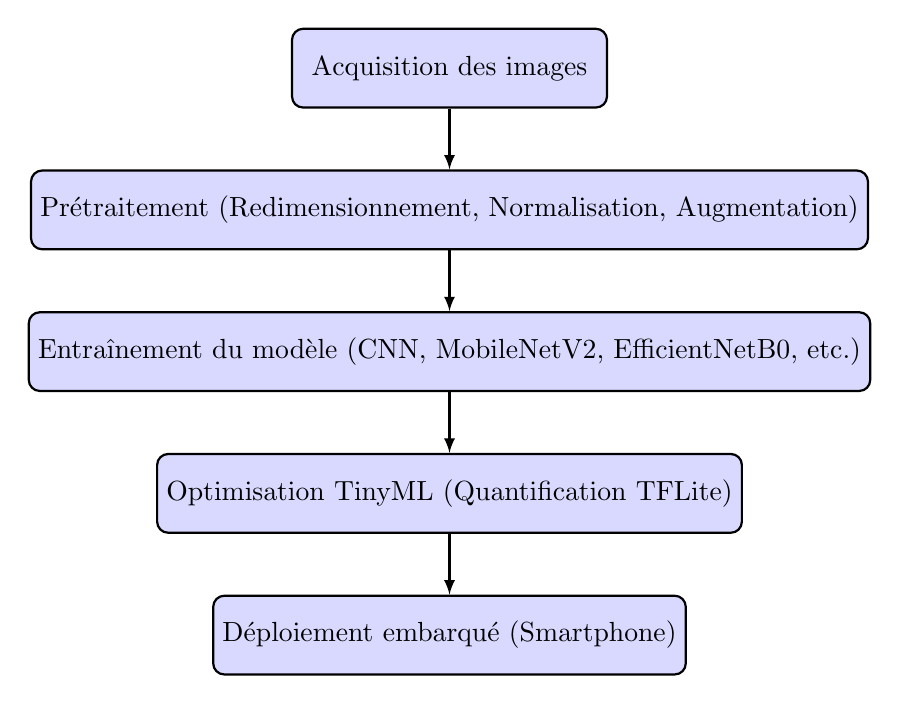
\begin{tikzpicture}[node distance=1.8cm, >=latex, thick]
      % Styles
      \tikzstyle{block} = [rectangle, draw=black, fill=blue!15, 
                          text centered, rounded corners, minimum width=4cm, minimum height=1cm]
      % Nodes
      \node[block] (acquisition) {Acquisition des images};
      \node[block, below of= acquisition] (pretraitement) {Prétraitement  (Redimensionnement, Normalisation, Augmentation)};
      \node[block, below of= pretraitement] (entrainement) {Entraînement du modèle  (CNN, MobileNetV2, EfficientNetB0, etc.)};
      \node[block, below of= entrainement] (optimisation) {Optimisation TinyML  (Quantification TFLite)};
      \node[block, below of= optimisation] (deploiement) {Déploiement embarqué  (Smartphone)};
      
      % Arrows
      \draw[->] (acquisition) -- (pretraitement);
      \draw[->] (pretraitement) -- (entrainement);
      \draw[->] (entrainement) -- (optimisation);
      \draw[->] (optimisation) -- (deploiement);
  \end{tikzpicture}
  \caption{Pipeline méthodologique proposé pour la prédiction du temps de cuisson des haricots basé sur TinyML.}
\end{figure}


  %%%%%%%%%%%%%%%%%%%%%%%%%%%%%%%%%%%%%%%%%%%%%%%%%%%%%%%%%%%%%%%%%%%%%%%%%%%%%%%%%%%%%%%%%%%%%%%%%%%%%%%%%%%%%%%%%%%%%%%%%%%%%%%%%%%%%%%%%%%%%%%%%%
  %%%%%%%%%%%%%%%%%%%%%%%%%%%%%%%%%%%%%%%%%%%%%%%%%%%%%%%%%%%%%%%%%%%%%%%%%%%%%%%%%%%%%%%%%%%%%%%%%%%%%%%%%%%%%%%%%%%%%%%%%%%%%%%%%%%%%%%%%%%%%%%%%%

  \section{Protocole expérimental — Prétraitement et préparation des jeux de données}

  Cette section détaille de façon exhaustive le protocole de prétraitement appliqué aux images et aux annotations de temps de cuisson ($T_c$), et précise la manière dont les jeux \emph{train/validation/test} sont construits et stockés pour l'entraînement et le déploiement TinyML.

  \subsection{Description synthétique du dataset source}

  Le jeu de données original comprend \(\mathbf{11\,200}\) images couleur au format JPEG, réparties équitablement sur \(\mathbf{8}\) variétés de haricots. Chaque variété est représentée par \(\mathbf{1\,400}\) images de haute résolution (\(3000\times4000\) pixels), répartie en \(\mathbf{7}\) sous-variétés contenant \(\mathbf{200}\) images chacune. Chaque image est associée à une annotation continue \(T_c\) (temps de cuisson en minutes), mesurée expérimentalement par chronométrage selon un protocole standardisé (arrêt au critère \emph{fork-tender}), avec une incertitude de mesure liée à l'opérateur estimée à \(\approx\pm 1\) minute.

  L’exploration préliminaire de la distribution des $T_c$ révèle une variabilité importante. Trois variétés présentent un pic de distribution autour de $120$ minutes, tandis que d'autres couvrent une plage de cuisson très large (approximativement de $70$ à $230$ minutes). Deux variétés en particulier montrent des profils de $T_c$ particulièrement étendus, ce qui souligne la nécessité d'une stratification rigoureuse lors du partitionnement des données pour garantir la représentativité de cette diversité dans chaque sous-ensemble.


  %%%%%%%%%%%%%%%%%%%%%%%%%%%%%%%%%%%%%%%%%%%%%%%%%%%%%%%%%%%%%%
  \subsection{Analyse Exploratoire et Statistiques Descriptives}

  Afin de caractériser quantitativement la distribution des données et d'orienter les choix de modélisation, une analyse exploratoire a été conduite \citep{tukey1977exploratory}. Cette analyse se concentre sur la distribution des temps de cuisson ($T_c$) à la fois globalement et au sein de chaque variété.

  %%%%%%%%%%%%%%%%%%%%%%%%%%%%%%%%%%%%%%%%%%%%%%%%%%%%%%%%%%%%%%
  \subsubsection{Statistiques descriptives par variété}

  Le tableau \ref{tab:stats_descriptives} résume les principaux descripteurs statistiques des temps de cuisson pour chaque variété.

  \begin{table}[!ht]
  \centering
  \caption{Statistiques descriptives des temps de cuisson ($T_c$ en minutes) par variété.}
  \label{tab:stats_descriptives}
  \begin{tabular}{lccccc}
  \toprule
  \textbf{Variété} & \textbf{Moyenne ($\mu$)} & \textbf{Écart-type ($\sigma$)} & \textbf{Min} & \textbf{Max} & \textbf{Effectif} \\ \midrule
  Dor701       & 145.86 & 72.67 & 62 & 280 & 1400 \\
  Escapan021   & 159.00 & 77.47 & 65 & 287 & 1400 \\
  GPL190C      & 160.00 & 74.19 & 70 & 295 & 1400 \\
  GPL190S      & 144.57 & 66.65 & 58 & 270 & 1400 \\
  Macc55       & 237.43 & 103.99 & 88 & 410 & 1400 \\
  NIT4G16187   & 118.86 & 45.18 & 68 & 210 & 1400 \\
  Senegalais   & 155.71 & 78.38 & 70 & 300 & 1400 \\
  TY339612     & 148.14 & 77.85 & 51 & 286 & 1400 \\ \bottomrule
  \end{tabular}
  \end{table}

  L'analyse de ces statistiques révèle plusieurs points cruciaux :
  \begin{itemize}
      \item \textbf{Forte hétérogénéité inter-variétés :} La moyenne des temps de cuisson varie considérablement, allant de $118.86$ min (NIT4G16187) à $237.43$ min (Macc55). Cette différence de plus de 100\% confirme que la variété est un facteur prédictif majeur du temps de cuisson.
      \item \textbf{Dispersion variable :} L'écart-type ($\sigma$), qui mesure la dispersion des valeurs autour de la moyenne, est également très hétérogène. La variété \texttt{Macc55} présente la plus forte dispersion ($\sigma \approx 104$ min), indiquant que ses temps de cuisson sont très étalés. À l'opposé, \texttt{NIT4G16187} est la plus homogène ($\sigma \approx 45$ min). Cette information est vitale : le modèle d'apprentissage pourrait avoir plus de difficultés à prédire avec précision le $T_c$ pour des variétés à forte variance.
      \item \textbf{Distribution globale :} La plage globale des temps de cuisson s'étend de 51 à 410 minutes, ce qui représente un défi de régression considérable pour un modèle TinyML contraint en ressources.
  \end{itemize}

  L'histogramme de la Figure \ref{fig:histogramme_tc} visualise la distribution globale des temps de cuisson, confirmant la présence de plusieurs modes et une asymétrie à droite.

  \begin{figure}[!ht]
  \centering
  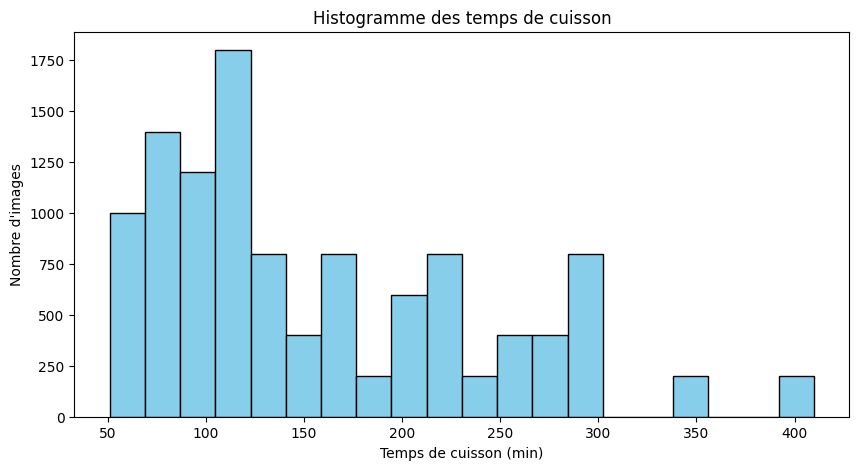
\includegraphics[width=0.8\textwidth]{figures/histogramme_tc.png}
  \caption{Distribution globale des temps de cuisson ($T_c$) pour l'ensemble des variétés. La distribution est multimodale, avec un pic principal autour de 120-150 minutes.}
  \label{fig:histogramme_tc}
  \end{figure}

  \subsubsection{Analyse de la variance intra-variété}

  Pour affiner l'analyse de la dispersion, la variance ($s^2 = \sigma^2$) a été calculée pour chaque variété (Tableau \ref{tab:variance_intra}). La variance quantifie la dispersion quadratique moyenne et accentue les différences de variabilité.

  \begin{table}[!ht]
  \centering
  \caption{Variance intra-variété des temps de cuisson.}
  \label{tab:variance_intra}
  \begin{tabular}{lc}
  \toprule
  \textbf{Variété} & \textbf{Variance Intra-variété ($s^2$)} \\ \midrule
  Dor701       & 5280.47 \\
  Escapan021   & 6002.00 \\
  GPL190C      & 5503.93 \\
  GPL190S      & 4442.28 \\
  Macc55       & 10813.97 \\
  NIT4G16187   & 2041.58 \\
  Senegalais   & 6143.16 \\
  TY339612     & 6060.17 \\ \bottomrule
  \end{tabular}
  \end{table}

  La Figure \ref{fig:boxplot_tc} (diagramme en boîtes à moustaches) offre une représentation visuelle comparative de ces variances. Elle met en évidence la médiane, l'intervalle interquartile (IQR) et l'étendue des données pour chaque catégorie, facilitant l'identification des distributions symétriques, asymétriques et des valeurs potentiellement aberrantes.

  \begin{figure}[!ht]
  \centering
  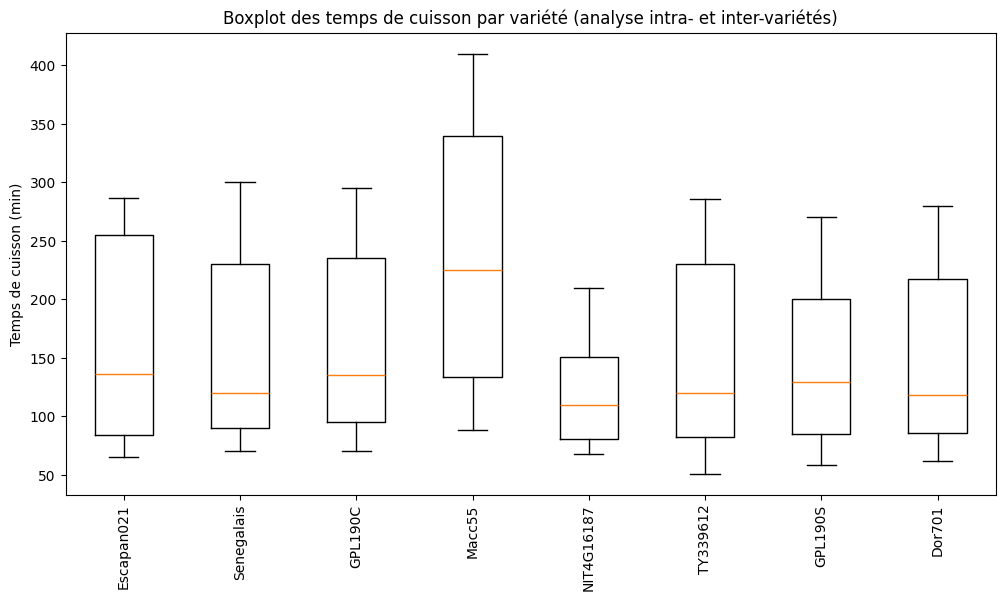
\includegraphics[width=0.9\textwidth]{figures/boxplot_tc.png}
  \caption{Diagramme en boîtes à moustaches illustrant la distribution des temps de cuisson par variété. La variabilité extrême de la variété \texttt{Macc55} et l'homogénéité de \texttt{NIT4G16187} sont clairement visibles.}
  \label{fig:boxplot_tc}
  \end{figure}

  L'examen de la variance et du boxplot confirme que la variété \texttt{Macc55} est un cas d'étude particulièrement difficile en raison de sa dispersion interne massive. Des facteurs non contrôlés, tels qu'une plus grande hétérogénéité génétique ou des conditions de croissance/stockage variables au sein de cette variété, pourraient expliquer ce phénomène. Du point de vue de la modélisation, cela implique que les caractéristiques visuelles extraites des images de \texttt{Macc55} doivent être particulièrement discriminantes pour permettre une régression précise.

  \subsubsection{Équilibre et distribution des données}

  La performance et l'impartialité d'un modèle d'apprentissage profond dépendent fortement de l'équilibre du jeu de données. La Figure \ref{fig:distrib_varietes} montre la répartition des échantillons par variété.

  \begin{figure}[!ht]
  \centering
  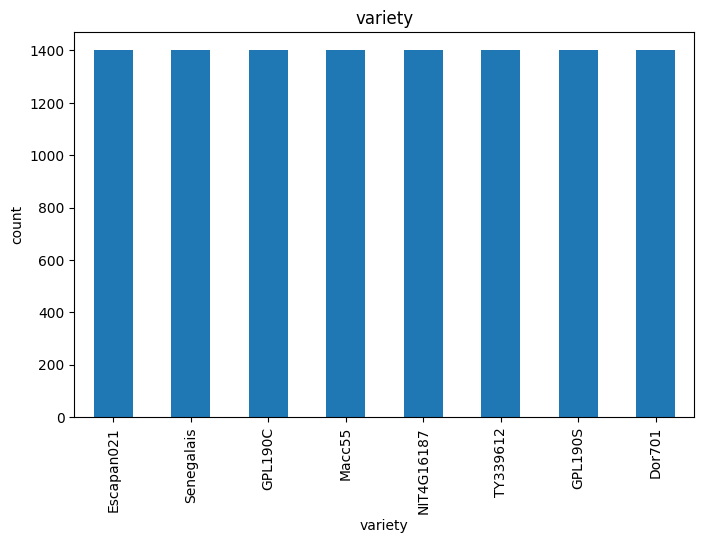
\includegraphics[width=0.7\textwidth]{figures/distrib_varietes.png}
  \caption{Distribution du nombre d'images par variété. Le jeu de données est parfaitement équilibré, chaque classe contenant 200 échantillons.}
  \label{fig:distrib_varietes}
  \end{figure}

  Le jeu de données est \textbf{parfaitement équilibré}, avec 200 images par variété. Cet équilibre est un atout majeur car il prévient tout biais du modèle en faveur des classes sur-représentées. La performance évaluée sera donc une juste réflexion de la capacité du modèle à généraliser sur toutes les variétés.


  \subsection{Pipeline de prétraitement}

  Le prétraitement appliqué aux images et aux annotations suit le pipeline illustré par la Figure \ref{fig:pipeline_preproc}. Seules les opérations jusqu'à l'enregistrement des jeux HDF5 sont incluses (préparation \textbf{offline} avant entraînement).

  \begin{figure}[H]
  \centering
  \begin{tikzpicture}[
    >=Latex,
    node distance=2.0cm,
    block/.style={rectangle, rounded corners=3pt, draw=black, fill=blue!12, align=center, minimum width=4.5cm, minimum height=0.9cm}
  ]
  \node[block] (raw) {Acquisition: images JPEG (3000×4000 px) \\ Labels: $T_c$ chronométrés};
  \node[block, below of=raw] (crop) {Recadrage centré / Ajustement d'exposition};
  \node[block, below of=crop] (resize) {Redimensionnement à 224×224 (PyTorch)};
  \node[block, below of=resize] (normalize_tc) {MinMax scaling de $T_c \to [0,1]$};
  \node[block, below of=normalize_tc] (augment) {Augmentation (train uniquement) $\times5$ \\ (flips, jitter, blur, noise)};
  \node[block, below of=augment] (h5) {Sauvegarde: un fichier HDF5 par split \\ clefs: \texttt{images}, \texttt{cooking\_times}};
  \draw[->] (raw) -- (crop);
  \draw[->] (crop) -- (resize);
  \draw[->] (resize) -- (normalize_tc);
  \draw[->] (normalize_tc) -- (augment);
  \draw[->] (augment) -- (h5);
  \end{tikzpicture}
  \caption{Pipeline de prétraitement des images et des labels $T_c$.}
  \label{fig:pipeline_preproc}
  \end{figure}

  \subsection{Redimensionnement et outils}

  Le redimensionnement est réalisé via \texttt{torchvision.transforms} (PyTorch) en appliquant un \texttt{CenterCrop} suivi d'un \texttt{Resize(224)} puis d'une normalisation des canaux si nécessaire pour des modèles pré-entraînés. Le choix $224\times224$ découle d'un compromis entre fidélité des motifs et coût mémoire d'inférence (MobileNetV2 / EfficientNet-B0 compatible) \citep{sandler2018mobilenetv2,krizhevsky2012imagenet}.

  \subsection{Augmentation (train uniquement) — paramètres}

  L'ensemble d'entraînement est étendu par un facteur $\mathbf{5}$ via des transformateurs aléatoires appliqués uniquement au split \emph{train} :
  \begin{itemize}
      \item \textbf{Flips horizontal et vertical} aléatoires ($p=0.5$),
      \item \textbf{RandomResizedCrop} (zoom et recadrage aléatoire),
      \item \textbf{ColorJitter} (variation de luminosité, contraste, saturation),
      \item \textbf{GaussianBlur} (flou gaussien léger),
      \item \textbf{Bruit Gaussien Additif}.
  \end{itemize}
  \textbf{Aucune rotation} n'est utilisée pour préserver les caractéristiques morphologiques directionnelles des grains. Ces transformations sont codées en PyTorch et appliquées stochastiquement pour générer quatre variantes supplémentaires par image d'entraînement initiale (1 image originale + 4 augmentées = facteur 5).

  \subsection{Normalisation des temps de cuisson ($T_c$)}

  Avant sauvegarde, les valeurs $T_c$ (en minutes) sont mises à l'échelle par la transformation \emph{Min–Max} pour produire une cible dans l'intervalle $[0,1]$. Formellement, les paramètres de la transformation sont calculés \textbf{uniquement} sur l'ensemble d'entraînement $\mathcal{D}_{\text{train}}$:

  \[
  T_{c,\min} = \min_{y\in \mathcal{D}_{\text{train}}} y, \qquad
  T_{c,\max} = \max_{y\in \mathcal{D}_{\text{train}}} y,
  \]
  \[
  \tilde{y} \;=\; \frac{y - T_{c,\min}}{T_{c,\max} - T_{c,\min}} \quad\in[0,1].
  \]

  Les mêmes $T_{c,\min}$ et $T_{c,\max}$ sont ensuite utilisés pour normaliser les ensembles de validation et de test, évitant ainsi toute fuite d'information du futur vers le modèle. Les valeurs prédites $\tilde{y}$ sont restaurées dans l'échelle d'origine (en minutes) par la transformation inverse $y = \tilde{y}\,(T_{c,\max}-T_{c,\min}) + T_{c,\min}$ lors de l'interprétation finale des résultats.

  \section{Conception du système proposé}

  La problématique adressée consiste à estimer, à partir d'une image unique d’un haricot (ou d'un petit lot représenté sur l'image), le temps de cuisson \(T_c\) exprimé en minutes. Le système doit être d'abord compétitif en termes de précision prédictive, puis contrainte à des ressources embarquées (smartphone et/ou microcontrôleur) via des techniques TinyML. La présente section décrit l'architecture générale et le pipeline de traitement, les modèles testés (deux CNN personnalisés et trois modèles préentraînés adaptés au mobile), les optimisations TinyML appliquées, ainsi que le workflow et l'architecture logicielle menant au déploiement.

  \subsection{Motivation et choix d'approche}

  L'approche par vision (images) est motivée par la possibilité d'extraire des indices visuels corrélés au temps de cuisson — couleur, taille, texture, proportion d'imperfections, etc. — sans recourir à des capteurs supplémentaires. Le passage à TinyML est justifié par l'objectif d'un service embarqué (hors-connexion) : confidentialité, latence faible et coût énergétique réduit. Les techniques d'optimisation (quantification, pruning, distillation) sont des bonnes pratiques largement documentées pour adapter des réseaux convolutifs classiques à des plateformes contraignantes \parencite{warden2019tinyml,Han2016DeepCompression}.

  \subsection{Architecture générale du modèle et pipeline}

  Le pipeline se décompose en quatre grandes phases (Figure~\ref{fig:pipeline}) :

  \begin{enumerate}
    \item \textbf{Prétraitement \& chargement} : lecture des HDF5, batch sampling, conversion en float32, normalisation canaux (mean/std) compatible avec les poids pré-entraînés ; augmentation appliquée uniquement au jeu d'entraînement.
    \item \textbf{Entraînement / Fine-tuning} : entraînement des CNN personnalisés depuis zéro et fine-tuning des modèles pré-entraînés (MobileNetV2, EfficientNet-B0, NASNetMobile) sur la tâche de régression continue (prévision du \(T_c\) normalisé).
    \item \textbf{Optimisation TinyML} : quantification (post-training et/ou quantization-aware training), pruning graduel, éventuellement distillation depuis un « teacher » plus large vers un « student » compact.
    \item \textbf{Déploiement \& mesures} : conversion en TFLite, mesures de latence et consommation sur smartphone cible (mesures empiriques, idéalement sur plusieurs appareils).
  \end{enumerate}

  \begin{figure}[!ht]
  \centering
  \begin{tikzpicture}[node distance=1.6cm, auto, >=Latex, thick]
  \tikzstyle{block} = [rectangle, rounded corners, draw, fill=blue!12, text centered, minimum height=1cm, minimum width=3.4cm]
  \node[block] (hdf5) {Chargement : HDF5 (train/val/test)};
  \node[block, below of=hdf5] (prep) {Normalisation des images};
  \node[block, below of=prep] (train) {Entraînement / Fine-tuning};
  \node[block, below of=train] (opt) {Quantification \& Pruning};
  \node[block, below of=opt] (deploy) {TFLite - Déploiement mobile};
  \draw[->] (hdf5) -- (prep);
  \draw[->] (prep) -- (train);
  \draw[->] (train) -- (opt);
  \draw[->] (opt) -- (deploy);
  \end{tikzpicture}
  \caption{Pipeline fonctionnel du système (chargement → entraînement → optimisation → déploiement).}
  \label{fig:pipeline}
  \end{figure}

  La fonction apprise s’écrit :
  \[
  \hat{T}_c = f_\theta\big(\mathcal{A}(I)\big)
  \]
  où \(I\in \mathbb{R}^{H\times W \times 3}\) est l'image d'entrée, \(\mathcal{A}\) l'opérateur de prétraitement (crop, resize à \(224\times224\), normalisation), et \(\theta\) les paramètres entraînés.

  \subsection{Description détaillée des modèles testés}

  Nous évaluons deux architectures convolutionnelles construites ad hoc (CNN-1 et CNN-2) et trois modèles mobiles pré-entraînés.

  \subsubsection{Formules de complexité et paramètres}

  Pour une couche convolutionnelle standard (sans séparabilité), le nombre de paramètres \(P\) et le nombre d'opérations élémentaires en multiplications-additions (FLOPs approximés par \emph{mult-adds}) pour une seule couche sont :
  \[
  P = (K \times K \times C_{in} + 1)\times C_{out},
  \]
  \[
  \text{FLOPs}_{\text{conv}} \approx 2 \times K \times K \times C_{in} \times C_{out} \times H_{out} \times W_{out},
  \]
  où \(K\) est la taille du noyau, \(C_{in},C_{out}\) canaux d'entrée/sortie et \(H_{out}\times W_{out}\) la résolution de la carte de caractéristiques en sortie (le facteur 2 approximant multiplication + addition). Pour les couches depthwise separable (utilisées par MobileNet), la complexité diminue sensiblement, ce qui explique l'efficacité de ces architectures sur mobile \citep{sandler2018mobilenetv2}.

  \subsubsection{CNN personnalisés (architectures fournies)}

\paragraph{CNN-1 TB-Net2 (profondeur progressive)}
L’architecture illustrée à la \textbf{Figure~\ref{fig:cnn1_tbnet2}} correspond à une approche dite de profondeur progressive, où le nombre de filtres est augmenté graduellement à mesure que la profondeur du réseau croît. Cette conception vise à extraire, dans un premier temps, des caractéristiques locales simples (bords, textures élémentaires), puis à capturer des représentations plus abstraites et discriminantes au fur et à mesure que les couches s’empilent.  

Chaque bloc convolutionnel est suivi d’une opération de sous-échantillonnage (\textit{MaxPooling2D}), qui réduit la résolution spatiale des cartes de caractéristiques tout en préservant les informations les plus saillantes. Cette stratégie permet de limiter la taille des tenseurs intermédiaires et d’augmenter l’invariance aux translations. L’intégration de couches de \textit{Dropout} avec un taux de 0.3 constitue un mécanisme de régularisation essentiel : elle réduit le risque de surapprentissage en introduisant une désactivation aléatoire de neurones lors de l’entraînement.  

Après plusieurs étapes de convolution et de pooling, une couche de \textit{GlobalAveragePooling2D} condense les cartes de caractéristiques en un vecteur représentatif, réduisant ainsi la dimensionnalité et favorisant la généralisation. Enfin, la partie dense est constituée d’une couche de 256 neurones activés par ReLU, suivie d’une couche de sortie unique adaptée à la régression du temps de cuisson.  

Dans l’ensemble, cette topologie offre un compromis pertinent entre expressivité et complexité computationnelle, en exploitant la profondeur pour raffiner progressivement l’information tout en maintenant une régularisation efficace.  

\begin{figure}[H]
    \centering
    \small
    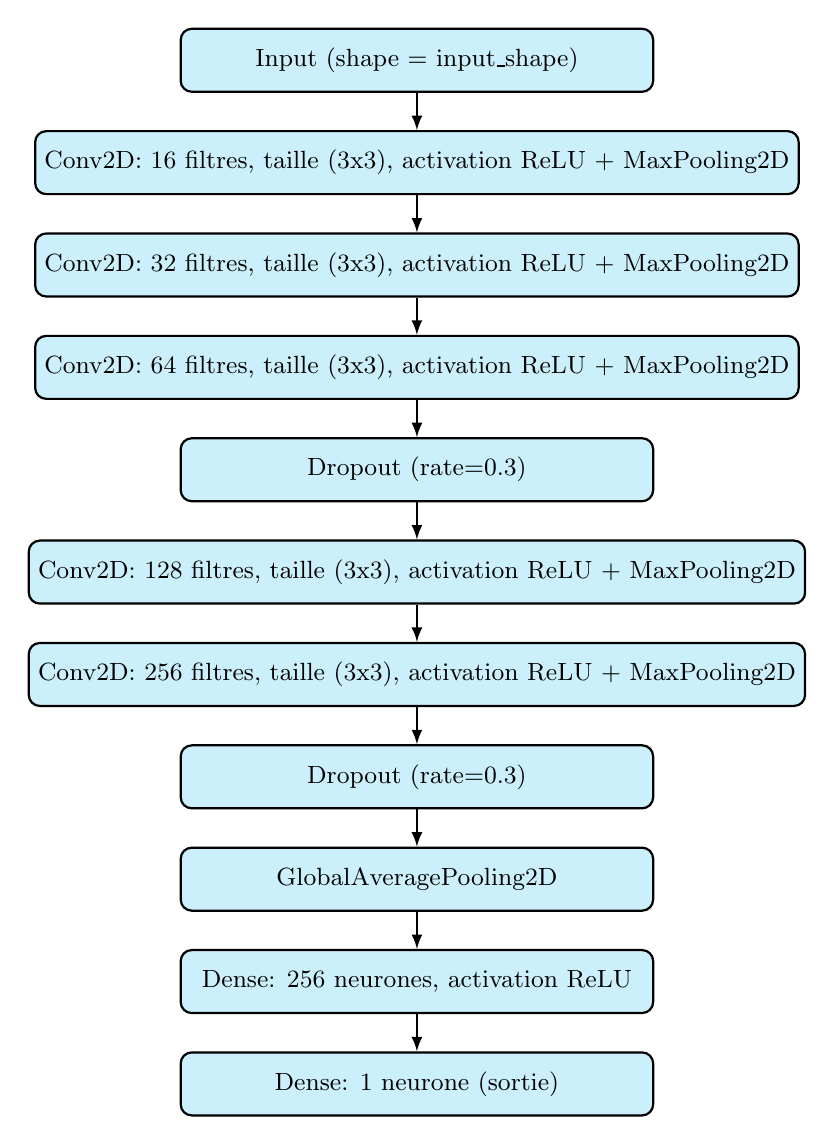
\begin{tikzpicture}[node distance=1.3cm, thick, >=latex, font=\small]
        \tikzstyle{block} = [rectangle, draw=black, fill=cyan!20, 
                            text centered, rounded corners, minimum width=6cm, minimum height=0.8cm]

        % Noeuds combinés Conv2D + MaxPooling2D
        \node[block] (input) {Input (shape = input\_shape)};
        \node[block, below of = input] (conv_pool1) {Conv2D: 16 filtres, taille (3x3), activation ReLU + MaxPooling2D};
        \node[block, below of = conv_pool1] (conv_pool2) {Conv2D: 32 filtres, taille (3x3), activation ReLU + MaxPooling2D};
        \node[block, below of = conv_pool2] (conv_pool3) {Conv2D: 64 filtres, taille (3x3), activation ReLU + MaxPooling2D};
        \node[block, below of = conv_pool3] (dropout1) {Dropout (rate=0.3)};
        \node[block, below of = dropout1] (conv_pool4) {Conv2D: 128 filtres, taille (3x3), activation ReLU + MaxPooling2D};
        \node[block, below of = conv_pool4] (conv_pool5) {Conv2D: 256 filtres, taille (3x3), activation ReLU + MaxPooling2D};
        \node[block, below of = conv_pool5] (dropout2) {Dropout (rate=0.3)};
        \node[block, below of = dropout2] (gap) {GlobalAveragePooling2D};
        \node[block, below of = gap] (dense1) {Dense: 256 neurones, activation ReLU};
        \node[block, below of = dense1] (output) {Dense: 1 neurone (sortie)};

        % Flèches
        \draw[->] (input) -- (conv_pool1);
        \draw[->] (conv_pool1) -- (conv_pool2);
        \draw[->] (conv_pool2) -- (conv_pool3);
        \draw[->] (conv_pool3) -- (dropout1);
        \draw[->] (dropout1) -- (conv_pool4);
        \draw[->] (conv_pool4) -- (conv_pool5);
        \draw[->] (conv_pool5) -- (dropout2);
        \draw[->] (dropout2) -- (gap);
        \draw[->] (gap) -- (dense1);
        \draw[->] (dense1) -- (output);
    \end{tikzpicture}
    \caption{Architecture CNN proposée avec blocs Conv2D et MaxPooling2D combinés.}
    \label{fig:cnn1_tbnet2_combined}
\end{figure}


\paragraph{CNN-2 TB-Net5 (bande passante accrue)}
L’architecture représentée à la \textbf{Figure~\ref{fig:cnn2_tbnet5}} se distingue du modèle précédent (CNN-1) par une augmentation significative de la largeur et de la profondeur des couches convolutionnelles. Alors que le premier réseau privilégiait une progression graduelle et régulière, ce second design adopte une stratégie d’expansion plus agressive du nombre de filtres, atteignant jusqu’à 512 dans les couches les plus profondes. Cette « bande passante accrue » confère au modèle une capacité de représentation plus riche, lui permettant de capturer des motifs complexes et subtils présents dans les images de haricots.  

Chaque bloc est constitué d’une couche \textit{Conv2D} suivie d’un \textit{MaxPooling2D}, assurant à la fois l’extraction de caractéristiques discriminantes et la réduction progressive de la résolution spatiale. La succession de ces blocs favorise une hiérarchisation efficace des représentations, allant des textures locales aux structures globales. L’intégration d’une couche de \textit{GlobalAveragePooling2D} avant la partie dense permet de condenser l’information tout en limitant la dimensionnalité des vecteurs de sortie.  

Enfin, une couche dense intermédiaire de 256 neurones activés par ReLU prépare les données avant la couche de sortie unique, adaptée à la régression du temps de cuisson. Bien que cette architecture soit plus coûteuse en termes de paramètres et d’opérations (FLOPs), elle est particulièrement pertinente lorsqu’une puissance de calcul suffisante est disponible, ou comme modèle « enseignant » dans une approche de distillation de connaissances en vue d’optimiser des variantes plus légères.  


\begin{figure}[H]
    \centering
    \small
    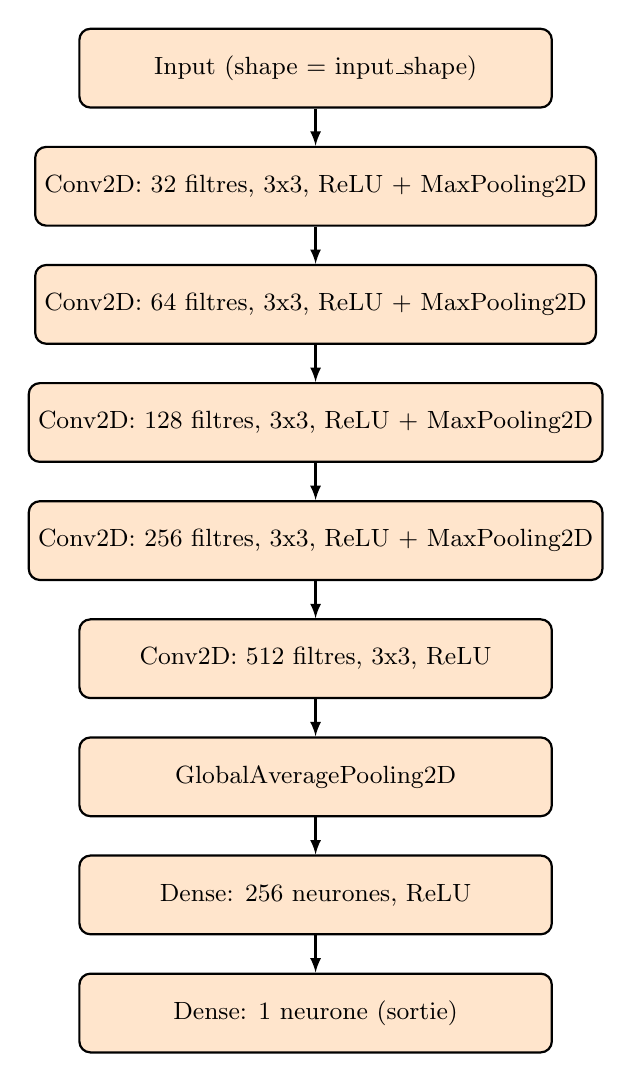
\begin{tikzpicture}[node distance=1.5cm, thick, >=latex, font=\small]
        \tikzstyle{block} = [rectangle, draw=black, fill=orange!20, 
                            text centered, rounded corners, minimum width=6cm, minimum height=1cm]

        % Noeuds combinés Conv2D + MaxPooling2D
        \node[block] (input) {Input (shape = input\_shape)};
        \node[block, below of = input] (conv_pool1) {Conv2D: 32 filtres, 3x3, ReLU + MaxPooling2D};
        \node[block, below of = conv_pool1] (conv_pool2) {Conv2D: 64 filtres, 3x3, ReLU + MaxPooling2D};
        \node[block, below of = conv_pool2] (conv_pool3) {Conv2D: 128 filtres, 3x3, ReLU + MaxPooling2D};
        \node[block, below of = conv_pool3] (conv_pool4) {Conv2D: 256 filtres, 3x3, ReLU + MaxPooling2D};
        \node[block, below of = conv_pool4] (conv5) {Conv2D: 512 filtres, 3x3, ReLU};
        \node[block, below of = conv5] (gap) {GlobalAveragePooling2D};
        \node[block, below of = gap] (dense1) {Dense: 256 neurones, ReLU};
        \node[block, below of = dense1] (output) {Dense: 1 neurone (sortie)};

        % Flèches
        \draw[->] (input) -- (conv_pool1);
        \draw[->] (conv_pool1) -- (conv_pool2);
        \draw[->] (conv_pool2) -- (conv_pool3);
        \draw[->] (conv_pool3) -- (conv_pool4);
        \draw[->] (conv_pool4) -- (conv5);
        \draw[->] (conv5) -- (gap);
        \draw[->] (gap) -- (dense1);
        \draw[->] (dense1) -- (output);
    \end{tikzpicture}
    \caption{Architecture CNN profonde avec blocs Conv2D et MaxPooling2D combinés.}
    \label{fig:cnn2_tbnet5_combined}
\end{figure}



  \subsubsection{Modèles pré-entraînés}

  \begin{itemize}
    \item \textbf{MobileNetV2} \parencite{sandler2018mobilenetv2} : architecture mobile employant des \emph{inverted residual} blocks et les convolutions séparables en profondeur ; MobileNetV2 (1.0, résolution 224) compte environ \(\mathbf{3.4M}\) paramètres et ~\(\mathbf{0.3}\) GFLOPs (mult-adds) pour une image 224×224, ce qui le rend très attractif pour l'embarqué.
    \item \textbf{EfficientNet-B0} \autocite{tan2019efficientnet} : conception via compound scaling ; EfficientNet-B0 : ~\(\mathbf{5.3M}\) paramètres et \(\approx\mathbf{0.39}\) GFLOPs (224×224). Excellente efficacité paramétrique/accuracie.
    \item \textbf{NASNetMobile} \autocite{zoph2018nasnet} : architecture trouvée par Neural Architecture Search pour des plateformes mobiles ; configurations compactes (taille et FLOPs compatibles avec mobile, ordre de quelques millions de paramètres selon l'implémentation).
  \end{itemize}

  Les nombres de paramètres et FLOPs cités ci-dessus proviennent des rapports originaux et benchmarks comparatifs (cf. Table~\ref{tab:model_comp} pour un résumé et les sources) \autocite{tan2019efficientnet,sandler2018mobilenetv2,zoph2018nasnet}.

  \subsection{Optimisations TinyML : quantification, pruning et techniques complémentaires}

  \subsubsection{Quantification}

  La quantification réduit la représentation numérique des poids et activations (fp32 → int8 ou fp16). La quantification post-training (PTQ) et la quantification-aware training (QAT) permettent d’obtenir des modèles 4× plus petits (int8) avec une perte de précision maîtrisée, surtout si l’on utilise une calibration dataset \autocite{jacob2018quantization,tensorflowlitequant}. TensorFlow Lite propose plusieurs variantes (dynamic range, full integer, float16) et outils pour mesurer l'impact \autocite{tensorflowlitequant}. 

  Mémoire approximative après quantification :
  \[
  \text{Taille}_{\text{int8}} \approx \frac{1}{4}\,\text{Taille}_{\text{fp32}}.
  \]
  Ex. : modèle fp32 12\,MiB \(\rightarrow\) int8 \(\approx\) 3\,MiB.

  \subsubsection{Pruning (élagage)}

  Le pruning structurel ou non-structurel supprime des poids ou canaux peu contributifs. En pratique, on applique un schéma de pruning itératif pendant l'entraînement et un ré-entraînement (fine-tuning) après pruning pour récupérer la performance \autocite{hinton2015distillation}. Les gains en mémoire et latence dépendent fortement de l'implémentation matérielle (le pruning non-structuré n'est pas toujours accéléré par le matériel généraliste).

  \subsubsection{Distillation de connaissances}

  Pour réduire davantage la taille tout en conservant la performance, on peut distiller un réseau compact (student) à partir d'un réseau plus large (teacher) — méthode particulièrement utile si l’on entraîne un petit CNN (CNN-2 ou CNN-1 après pruning) pour produire un modèle embarquable \autocite{hinton2015distillation}.

  \subsection{Workflow expérimental et hyperparamètres}

  Nous suivons une procédure reproductible incluant des scripts d'entraînement, conversion et test. Le tableau~\ref{tab:hyper} résume les hyperparamètres recommandés pour l'expérimentation initiale ; ces valeurs servent de baseline et peuvent être optimisées par recherche (grid/random/Bayesian).

  \begin{table}[!ht]
  \centering
  \caption{Hyperparamètres d'entraînement recommandés.}
  \label{tab:hyper}
  \resizebox{\textwidth}{!}{%
  \begin{tabular}{@{}lcc@{}}
  \toprule
  Hyperparamètre & Valeur (baseline) & Commentaire \\ \midrule
  Batch size & 32 & adapter selon VRAM GPU \\
  Optimiseur & Adam & \(\beta_1=0.9, \beta_2=0.999\) \\
  Learning rate init. & $10^{-4}$ & scheduler Cosine decay ou ReduceOnPlateau \\
  Epochs & 100 & early stopping sur val loss (patience 5) \\
  Loss & MSE (régression) & on suit MAE/MAPE en métriques secondaires \\
  Augmentation (train) & flip, crop, color jitter, blur, bruit gaussien & multiplicateur ×5 \\
  Normalisation sorties & Min–Max (train) & transforme \(T_c\) en \([0,1]\) \\
  Quantification & PTQ int8 puis QAT si forte dégradation & calibration sur subset test \\
  Pruning & 30–60\% sparsité progressive & ré-entraînement post-pruning \\
  \bottomrule
  \end{tabular}%
  }
  \end{table}


  \subsection{Comparaison chxiffrée des modèles (estimation)}

  La Table~\ref{tab:model_comp} rassemble des métriques utiles pour comparer précision/complexité/taille : nombre de paramètres, FLOPs (mult-adds), taille indicative après quantification en int8, et latence attendue (estimation à valider empiriquement sur smartphone cible). Les valeurs de paramètres/FLOPs sont extraites des publications originales et benchmarks \autocite{sandler2018mobilenetv2,tan2019efficientnet,zoph2018nasnet, openbenchmarks}.

  \begin{table}[!ht]
  \centering
  \caption{Comparatif des modèles (valeurs indicatives pour 224×224).}
  \label{tab:model_comp}
  \begin{tabular}{@{}lcccc@{}}
  \toprule
  Modèle & \# Param. & FLOPs (G) & Taille float16 (est.) & Latence \\
  & (M) & (mult-adds) & (Mo) & (ms sur smartphone) \\ \midrule
  CNN-1 (config) &  \(\approx\) 1.38 & \(\approx\) 0.1 & 0.90 & 20--30\(^\dagger\) \\
  CNN-2 (config) &  \(\approx\) 5 & \(\sim\) 0.4--0.6 & 5 & 40--80\(^\dagger\) \\
  MobileNetV2 (1.0) & \(\approx\) 3.4 & \(\approx\) 0.3 & \(\approx\) 2.4--6.6 & 30--60\(^\dagger\) \\
  EfficientNet-B0 & \(\approx\) 5.3 & \(\approx\) 0.39 & \(\approx\) 2.8--5.5 & 40--80\(^\dagger\) \\
  NASNetMobile & \(\sim\) 4.0--6.0 & \(\sim\) 0.5--0.6 & \(\approx\) 3.0--7.0 & 50--100\(^\dagger\) \\ \bottomrule
  \end{tabular}
  \begin{flushleft}
  \footnotesize{\(^\dagger\) latences approximatives — très dépendantes du modèle exact, du téléphone (CPU, NNAPI), et de la présence d'accélération intégée. Mesures empiriques recommandées (cf. \autocite{tan2019efficientnet,sandler2018mobilenetv2,tan2019mnasnet}).}
  \end{flushleft}
  \end{table}

  \noindent \textbf{Note importante :} les chiffres indiqués sont des ordres de grandeur tirés de la littérature et de benchmarks publics ; il est impératif de mesurer la latence et la consommation sur la plateforme cible (par ex. instrumentation via Android Profiler, Systrace, ou outils d’energy profiling) pour obtenir des valeurs applicables \autocite{tan2019mnasnet}.

  \subsection{Intégration embarquée : smartphone, gestion mémoire, latence et consommation}

  \paragraph{Plateforme cible}  
  Le choix initial est le smartphone Android moderne (API >= 24) afin d'utiliser TensorFlow Lite et NNAPI pour l'accélération. Pour microcontrôleurs, la chaîne change (TFLite Micro, contraintes SRAM/Flash beaucoup plus strictes) ; Warden et Situnayake fournissent des guides pratiques pour Arduino/MCU \autocite{warden2019tinyml}.

  \paragraph{Mesures et profilage}  
  Mesures empiriques à effectuer :
  \begin{itemize}
    \item \textbf{Taille binaire du modèle} (apk ou fichier .tflite) avant/après quantification ;
    \item \textbf{Latence d'inférence} (cold start et warm runs) : moyenne et percentiles sur N exécutions ;
    \item \textbf{Consommation énergétique} (mJ) par inférence : via instrumentation matérielle (moniteur de courant) ou outils logicielles approximatives ;
    \item \textbf{Utilisation mémoire} (heap et allocation interne du runtime).
  \end{itemize}
  Ces mesures servent à comparer les modèles et à choisir le meilleur compromis précision/consommation/latence \autocite{tan2019mnasnet,fbnet}.

  \paragraph{Gestion mémoire et performance}  
  Quelques bonnes pratiques pour réduire l'empreinte :
  \begin{itemize}
    \item utiliser \texttt{delegate} matériels (NNAPI, GPU delegate) quand disponibles ;
    \item privilégier la quantification entière (int8) pour la réactivité CPU et la réduction mémoire \autocite{jacob2018quantization,tensorflowlitequant};
    \item s'assurer que les buffers d'entrée/sortie sont réutilisés pour éviter des allocations répétées ;
    \item appliquer pruning structurel pour réduire latence (canaux/filters pruning) plutôt que pruning non-structuré si l'accélération matérielle est limitée.
  \end{itemize}

  \subsection{Aspects reproductibilité et intégration continue}

  Le pipeline CI doit inclure :
  \begin{itemize}
    \item scripts pour recréer dataset HDF5 à partir des images (même random seed pour splits) ;
    \item étapes d'entraînement avec logging (TensorBoard), sauvegarde de checkpoints et export du modèle sauvegardé ;
    \item étapes automatisées de conversion TFLite + application des options de quantification (scripts identiques à ceux utilisés pour la production) ;
    \item tests unitaires validant que la sortie TFLite réplique la prédiction du modèle de référence (tolérance via MAE).
  \end{itemize}

  \subsection{Discussion critique et limites}

  \begin{itemize}
    \item \textbf{Variabilité inter-variétés} : la distribution des temps de cuisson varie fortement selon la variété (cf. protocole). Un modèle global peut sous-performer pour certaines variétés ; des stratégies incluent l'ajout d'un embedding de variété (si l'information est connue) ou l'entraînement de modèles spécialisés.
    \item \textbf{Sources d'erreur visuelle} : éclairage, positionnement, ombres peuvent dégrader les prédictions ; inclure des augmentations robustes et collecter des images représentatives en conditions réelles réduit ce risque.
    \item \textbf{Compromis précision/latence} : une petite perte de précision peut être acceptable si la latence et la consommation chutent significativement — décision à prendre selon contrainte d'usage (temps réel vs analyse batch).
  \end{itemize}

  La conception exposée ci-dessus fixe les choix techniques et les métriques d'évaluation nécessaires. Le chapitre suivant (Implémentation) détaillera la configuration expérimentale (scripts d'entraînement Keras/TensorFlow), les commandes de conversion TFLite (options de quantification), les protocoles de mesure sur smartphone et les résultats empiriques (MAE, RMSE, taille finale des modèles, latence et consommation mesurées).		
\chapter{Développement et implémentation}
\label{chap:developpement}

Ce chapitre présente la mise en œuvre concrète du système de prédiction du temps de cuisson des haricots, depuis la préparation des données jusqu’au déploiement embarqué. Il s’appuie sur la méthodologie définie au Chapitre~\ref{chap:methodologie} et reprend strictement les choix techniques (prétraitements, architectures candidates, schéma d’entraînement et optimisation TinyML).

\section{Environnement de développement}
\label{sec:env_dev}

\subsection{Matériel}
Les expérimentations ont été menées sur :
\begin{itemize}
	\item \textbf{Machine locale} : Intel Core i7 (4 cœurs), 16~Go RAM.
	\item \textbf{Google Colab} : session \texttt{Tesla T4} (15~Go VRAM, 12~Go RAM, 118~Go stockage).
	\item \textbf{Samsung Galaxy Note 9} : Octa-core, 6 Go RAM, 128~Go stockage, Android 10.
\end{itemize}

\subsection{Logiciels et versions}
Sauf mention contraire, les versions utilisées sont celles définies en méthodologie :
\begin{itemize}
	\item \textbf{Python} 3.10
	\item \textbf{TensorFlow} 2.19 pour l'entrainement et \textbf{TensorFlow} 2.13 pour la quantification \& API Keras (compatibles \texttt{TensorFlow Lite})
	\item \textbf{Pandas} 2.1, \textbf{NumPy} 1.25, \textbf{Matplotlib} 3.8
\end{itemize}

\section{Préparation des données}
\label{sec:pretraitement}

Le protocole de préparation suit \textit{strictement} le Chapitre~\ref{chap:methodologie} :
\begin{enumerate}
	\item \textbf{Recadrage centré} et \textbf{redimensionnement} des images brutes (\(3000\times4000\)) en \(224\times224\).
	\item \textbf{Mise à l’échelle} des pixels dans \([0,1]\).
	\item \textbf{Augmentation} stochastique \textit{train-only} (flips, crops, jitter de luminosité/contraste/saturation, blur, bruit gaussien)\footnote{Paramètres détaillés : voir Chap.~\ref{chap:methodologie}.}.
	\item \textbf{Normalisation Min--Max} des labels \(T_c\in[0,1]\), calculée uniquement sur \(\mathcal{D}_{\text{train}}\), appliquée à val/test, puis inversée pour restituer les minutes en sortie.
	\item \textbf{Export HDF5} par split avec clés \texttt{images}, \texttt{cooking\_times}.
\end{enumerate}

%%%%%%%%%%% Pré-entrainement %%%%%%%%%%%%%%%%%%%%%%%%%%%%%%%%%%%%%%%%%

\begin{verbatim}
\small
1. Charger le fichier CSV contenant les chemins d’images et les étiquettes (labels).
2. Extraire la liste des chemins d’images et convertir les labels au format float.
3. Définir les transformations de base (redimensionnement, conversion en tenseur).
4. Définir les transformations d’augmentation de données 
   (redimensionnement, recadrage aléatoire, flips, jitter couleur, flou gaussien).
5. Pour chaque chemin d’image :
    a. Ouvrir l’image et la convertir en RGB.
    b. Appliquer la transformation de base.
    c. Convertir l’image en tableau numpy uint8 et l’ajouter à la liste des images de base.
6. Convertir la liste des images et labels en tableaux numpy.
7. Normaliser les labels entre 0 et 1.
8. Séparer le jeu de données en ensembles d'entraînement, de validation et de test 
   (stratification sur les labels).
9. Pour chaque image de l’ensemble d’entraînement :
    a. Ajouter l’image originale et son label.
    b. Pour un nombre donné d’augmentations :
        i. Convertir l’image en format PIL.
       ii. Appliquer les transformations d’augmentation.
      iii. Convertir l’image augmentée au format numpy uint8.
       iv. Ajouter l’image augmentée et le label à la liste.
10. Convertir les listes d’images et labels augmentés en tableaux numpy.
11. Enregistrer chaque ensemble (entraînement, validation, test) dans un fichier HDF5, 
    avec deux jeux de données : images et labels (temps de cuisson).
\end{verbatim}

\section{Architectures de modèles}
\label{sec:modeles}

Conformément à la méthodologie :
\begin{itemize}
	\item \textbf{CNN personnalisés} (deux variantes) pour une extraction hiérarchique efficace.
	\item \textbf{MobileNetV2}, \textbf{EfficientNetB0}, \textbf{NASNetMobile} (apprentissage par transfert).
\end{itemize}

La tête de régression est composée d’une couche de sortie scalaire (\texttt{linear}).
La régularisation inclut un \texttt{dropout} de 0.3 et une pénalisation L2 (\(\lambda=10^{-4}\)).

%%%%%%%%%%% Tableau des hyperparamètres %%%%%%%%%%%%%%%%%%%%%%%%%%%%%%%%%%%%%%%%%
\begin{table}[h!]
	\centering
	\caption{Hyperparamètres d’entraînement retenus.}
	\label{tab:hyperparams}
	\begin{tabular}{l l}
		\toprule
		Paramètre                    & Valeur                                             \\ \midrule
		Optimiseur                   & Adam (\(\beta_1=0.9\), \(\beta_2=0.999\))          \\
		Taux d’apprentissage initial & \(10^{-4}\) + scheduler \texttt{ReduceLROnPlateau} \\
		Fonction de perte            & MSE                                                \\
		Métriques                    & MAE, RMSE, \(R^2\)                                 \\
		Batch size                   & 32                                                 \\
		Époques max                  & 100                                                \\
		Patience early stopping      & 5                                                  \\
		Dropout                      & 0.3                                                \\
		Régularisation L2            & \(10^{-4}\)                                        \\ \bottomrule
	\end{tabular}
\end{table}

\section{Stratégie d’entraînement}
\label{sec:entrainement}

Le modèle est entraîné sur \(\mathcal{D}_{\text{train}}\), validé sur \(\mathcal{D}_{\text{val}}\).
L’\textit{early stopping} permet d’éviter le surapprentissage.

%%%%%%%%%%%%%%%%%%%%%%%%%%%%%%% Fonction d'entrainement des modèles %%%%%%%%%%%%%%%%%%%%%%%%%%%%%%%
\begin{verbatim}
\small
1. Initialiser les variables pour la meilleure validation MAE et le compteur de patience.
2. Construire une nouvelle instance du modèle via la fonction model_builder.
3. Initialiser un dictionnaire pour stocker l’historique d’entraînement.
4. Charger le jeu de données d’entraînement à partir du chemin donné.
5. Calculer le nombre d’itérations (steps) par époque selon la taille du batch.
6. Pour chaque époque dans le nombre total d’époques :
    a. Afficher l’information de l’époque en cours.
    b. Créer un générateur de batchs d’entraînement.
    c. Entraîner le modèle sur une époque complète avec le générateur.
    d. Récupérer la perte (loss) et la MAE d’entraînement.
    e. Évaluer le modèle sur les données de validation pour obtenir val_loss et val_mae.
    f. Enregistrer ces métriques dans l’historique.
    g. Afficher un résumé des résultats d’entraînement et de validation.
    h. Appliquer une stratégie d’early stopping :
        i. Si val_mae s’améliore, sauvegarder le modèle et réinitialiser le compteur de patience.
       ii. Sinon, incrémenter le compteur de patience.
      iii. Si le compteur atteint la patience maximale, arrêter l’entraînement prématurément.
    i. Libérer la mémoire du générateur.
7. Afficher la fin de l’entraînement.
8. Fermer le loader de données.
9. Retourner l’historique d’entraînement.
\end{verbatim}

\section{Export et optimisation TinyML}
\label{sec:optim_tinyml}

\subsection{Conversion TensorFlow Lite (float16)}
La quantification retenue est \textbf{float16}, permettant de réduire la taille mémoire d’environ 50\% tout en préservant la précision.

%%%%%%%%%%%%%%%%%%%% Conversion du modèle %%%%%%%%%%%%%%%%%%%%%%%%%%%%%%%%%%%%%%%%
\begin{verbatim}
1. Importer la bibliothèque TensorFlow (version 2.13).
2. Charger le modèle enregistré (SavedModel).
3. Initialiser un convertisseur TFLite à partir du modèle chargé.
4. Activer les optimisations par défaut pour la conversion.
5. Spécifier que le type de données cible est float16 (pour Android).
6. Convertir le modèle en format TFLite.
7. Sauvegarder le modèle TFLite dans un fichier binaire.
8. Afficher un message de succès de la conversion.
\end{verbatim}

\section{Déploiement Android}
\label{sec:deploiement_android}

\subsection{Cible et outils}
\begin{itemize}
	\item \textbf{Android Studio} Narwhal (2025.1.2), \textbf{SDK} Android 36.
	\item Compatibilité descendante : \texttt{minSdkVersion=26} (Android 8.0).
	\item \textbf{Langage} : Kotlin.
	\item \textbf{Runtime ML} : \texttt{TensorFlow Lite Interpreter} v2.13.
\end{itemize}

\subsection{Intégration et inférence}
Le modèle \texttt{.tflite} est placé dans \texttt{assets/}.
Le pipeline embarqué applique le même prétraitement (resize \(224\times224\), normalisation), puis l’inférence, suivie de l’inversion Min--Max pour obtenir le temps en minutes.

%%%%%%%%%%%%%%%%%%%%% Deploiement sur Android %%%%%%%%%%%%%%%%%%%%%%%%%%%%%%
\begin{verbatim}
\small
1. MainViewModel (ViewModel) :
    - Définir états observables : imageBitmap, predictionResult.
    - Constantes : taille image (224x224), min/max temps cuisson.
    - loadModelFile(context, modelPath) : charger modèle TFLite depuis assets.
    - runPrediction(context, bitmap) :
        a. Mettre à jour imageBitmap et predictionResult.
        b. Lancer coroutine pour exécuter runModelInference.
        c. Mesurer latence et mettre à jour predictionResult.
        d. Gérer erreurs.
    - runModelInference(context, bitmap) :
        a. Convertir bitmap en ARGB_8888 si nécessaire.
        b. Redimensionner à 224x224.
        c. Créer ByteBuffer, normaliser pixels [0,1].
        d. Charger interpréteur TFLite.
        e. Exécuter inférence et récupérer sortie.
        f. Dénormaliser prédiction et retourner.
    - denormalize(normalizedValue) : convertir sortie normalisée en valeur réelle.
    - reset() : réinitialiser états.
2. IntroManager :
    - Gérer SharedPreferences pour écran d’introduction.
    - shouldShowIntro() : retourner booléen.
    - setShowIntro(shouldShow) : modifier préférence.
3. MainActivity :
    - Initialiser IntroManager.
    - Afficher IntroScreen si besoin, sinon écran prédiction.
    - Navigation entre PredictionScreen et InfoScreen.
4. Composables UI :
    - IntroScreen : boîte de dialogue avec option "ne plus afficher".
    - PredictionScreen :
        a. Gérer permissions caméra, sélection image galerie/camera.
        b. Afficher image sélectionnée.
        c. Afficher résultats prédiction (temps, RMSE, MAE).
        d. Boutons importer, prendre photo, réinitialiser.
    - InfoScreen :
        a. Présentation app.
        b. Explication métriques MAE et RMSE.
        c. Contexte cuisson haricots.
\end{verbatim}

\paragraph{UI/Workflow.}
\begin{figure}[H]
	\centering
	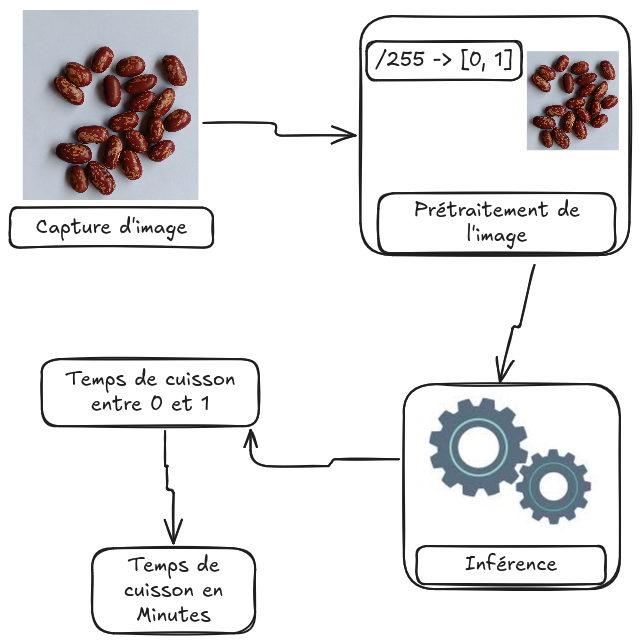
\includegraphics[width=0.9\textwidth]{figures/workflow.png}
	\caption{Workflow fonctionnel de l’application Android : capture ou import d’image, prétraitement, inférence et affichage du temps de cuisson (\(T_c\)).}
	\label{fig:app_workflow}
\end{figure}

\section{Mesures et artefacts à produire}
\label{sec:mesures_artefacts}

Cette section ne présente \emph{pas} de résultats chiffrés (qui seront rapportés au Chapitre Résultats), mais liste les artefacts générés.

\begin{table}[h!]
	\centering
	\caption{(Placeholder) Synthèse des modèles déployables.}
	\label{tab:deploy_synthese}
	\begin{tabular}{@{}lcccc@{}}
		\toprule
		Modèle         & Fichier TFLite     & Taille (Mo) & Latence (ms)\textsuperscript{$\dagger$} & Notes   \\ \midrule
		TBNet2         & model\_fp16.tflite & 0.9         & 187                                     & float16 \\
		MobileNetV2    & model\_fp16.tflite & 7.2         & 734                                     & float16 \\
		EfficientNetB0 & model\_fp16.tflite & 8.7         & 769                                     & float16 \\
		NASNetMobile   & model\_fp16.tflite & 21.3        & 867                                     & float16 \\ \bottomrule
	\end{tabular}
\end{table}

\footnotesize{$\dagger$ Mesures effectuées sur appareil cible (moyenne et percentiles).}

\section{Limites pratiques et points d’attention}
\label{sec:limites}
\begin{itemize}
	\item \textbf{Alignement des prétraitements} : le pipeline embarqué doit reproduire fidèlement la normalisation et l’inversion Min--Max.
	\item \textbf{Latence et consommation} : fortement dépendantes de l’appareil et des délégués (CPU/GPU/NNAPI).
	\item \textbf{Gestion mémoire} : réutilisation des buffers d’E/S et chargement paresseux recommandés côté Android.
	\item \textbf{Robustesse applicative} : prévoir la gestion des erreurs (fichier image invalide, absence d’entrée).
\end{itemize}

\bigskip
\noindent \textbf{Résumé} — Ce chapitre documente l’implémentation complète (prétraitement, modèles, entraînement, conversion float16, intégration Android) et définit les artefacts à produire. Les résultats expérimentaux seront présentés et analysés au Chapitre~\ref{chap:resultats_discussion}.
		
\chapter{Résultats et Discussion}
\label{chap:resultats_discussion}

Ce chapitre présente et analyse les résultats expérimentaux obtenus à partir des deux volets du système :
(i) la \textbf{classification des variétés de haricots}, et
(ii) la \textbf{régression du temps de cuisson}.
L’objectif est d’évaluer de manière approfondie les performances des modèles et de discuter de leurs limites, de leur robustesse et de leurs perspectives d’application.

\section{Résultats de la classification}
\label{sec:resultats_classification}

L’étape de classification a pour but d’identifier la variété de haricot à partir d’une image RGB.
Cette reconnaissance préalable conditionne la précision de la prédiction du temps de cuisson, car chaque variété présente des caractéristiques structurelles et biochimiques propres.

Le modèle de classification entraîné a atteint une \textbf{accuracy globale de 97\,\%} sur le jeu de test, traduisant une excellente capacité de généralisation.
Le Tableau~\ref{tab:classification_metrics} présente les résultats détaillés en termes de précision, rappel et F1-score pour chaque classe.

\begin{table}[H]
	\centering
	\caption{Performances de classification par variété de haricot.}
	\label{tab:classification_metrics}
	\begin{tabular}{|l|c|c|c|c|}
		\hline
		\textbf{Classe}        & \textbf{Précision}        & \textbf{Rappel} & \textbf{F1-score} & \textbf{Support} \\
		\hline
		Dor701                 & 1.00                      & 1.00            & 1.00              & 70               \\
		Escapan021             & 1.00                      & 0.96            & 0.98              & 70               \\
		GPL190C                & 0.90                      & 0.86            & 0.88              & 70               \\
		GPL190S                & 0.87                      & 0.94            & 0.90              & 70               \\
		Macc55                 & 1.00                      & 0.96            & 0.98              & 70               \\
		NIT4G16187             & 1.00                      & 1.00            & 1.00              & 70               \\
		Sénégalais             & 1.00                      & 1.00            & 1.00              & 70               \\
		TY339612               & 0.96                      & 1.00            & 0.98              & 70               \\
		Autre                  & 1.00                      & 1.00            & 1.00              & 200              \\
		\hline
		\textbf{Accuracy}      & \multicolumn{3}{c|}{0.97} & 760                                                    \\
		\textbf{Macro Avg.}    & 0.97                      & 0.97            & 0.97              & 760              \\
		\textbf{Weighted Avg.} & 0.97                      & 0.97            & 0.97              & 760              \\
		\hline
	\end{tabular}
\end{table}

La Figure~\ref{fig:matrice_confusion} illustre la matrice de confusion.
On y observe que la majorité des classes sont correctement identifiées, avec quelques confusions résiduelles entre \texttt{GPL190C} et \texttt{GPL190S}, deux variétés morphologiquement proches.

\begin{figure}[H]
	\centering
	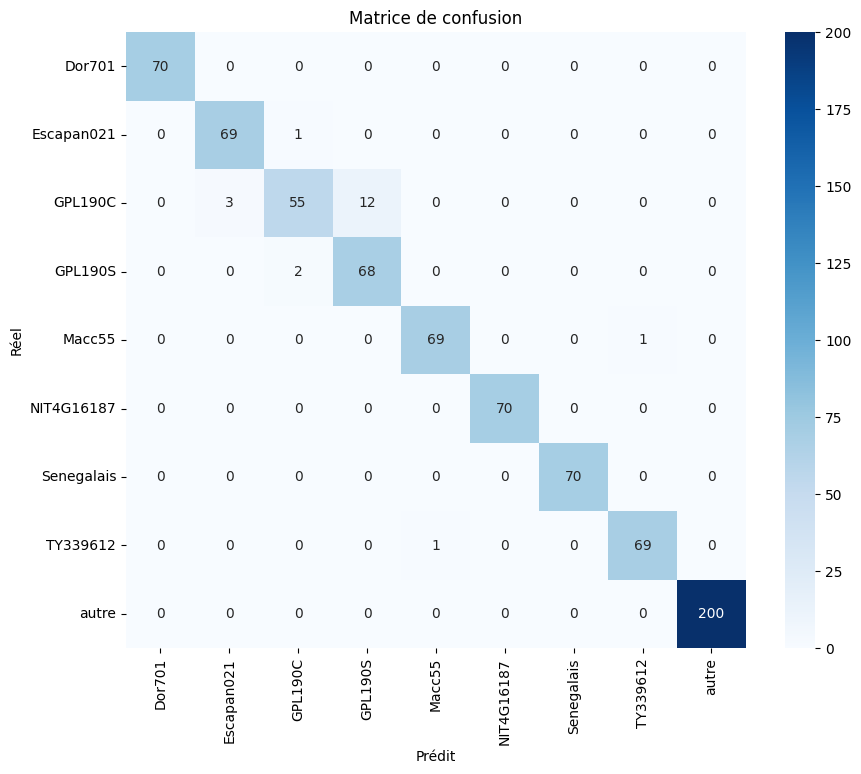
\includegraphics[width=0.75\textwidth]{figures/matrice_confusion.png}
	\caption{Matrice de confusion obtenue pour la classification des variétés de haricots.}
	\label{fig:matrice_confusion}
\end{figure}

\subsection{Analyse et comparaison à l’état de l’art}

Ces résultats confirment que des CNN compacts appliqués à des images RGB peuvent rivaliser avec des approches plus coûteuses en hyperspectral.
Par exemple, \cite{mohanty2016using} rapportent une précision de 98\,\% pour la classification de cultures agricoles, tandis que \cite{sladojevic2016deep} atteignent 96\,\% pour l’identification de maladies foliaires.
Dans le cas spécifique des graines, \cite{jiang2020cnn} montrent que les CNN surpassent les méthodes basées sur des caractéristiques manuelles (SIFT, HOG).

Ainsi, le modèle proposé, atteignant 97\,\% d’accuracy, se positionne dans la fourchette haute des performances rapportées dans la littérature, tout en étant optimisé pour une intégration future sur dispositifs embarqués.

\section{Résultats de la régression}
\label{sec:resultats_regression}

Après identification de la variété, le système estime le temps de cuisson en minutes.
L’évaluation repose sur les métriques classiques de régression : MAE, RMSE, $R^2$, MAPE et MaxErr.

\subsection{Courbes de perte et convergence des modèles}
\label{subsec:loss_curves}

Les modèles personnalisés \texttt{TBNet5} et \texttt{TBNet2} convergent rapidement, stabilisant la perte après 20–25 époques, contrairement aux modèles pré-entraînés qui présentent davantage de fluctuations.
Toutefois, \texttt{TBNet5} présente des signes d’\textit{overfitting} \cite{goodfellow2016deep} : sa perte de validation tend à stagner ou fluctuer malgré une amélioration continue de la perte d’entraînement.
De plus, sa taille mémoire et sa complexité sont significativement plus élevées que celles de \texttt{TBNet2}, ce qui limite son adéquation aux environnements contraints.

À performances quasi équivalentes, \texttt{TBNet2} constitue donc le meilleur compromis et a été retenu comme modèle final pour la suite des analyses.

\begin{figure}[H]
	\centering
	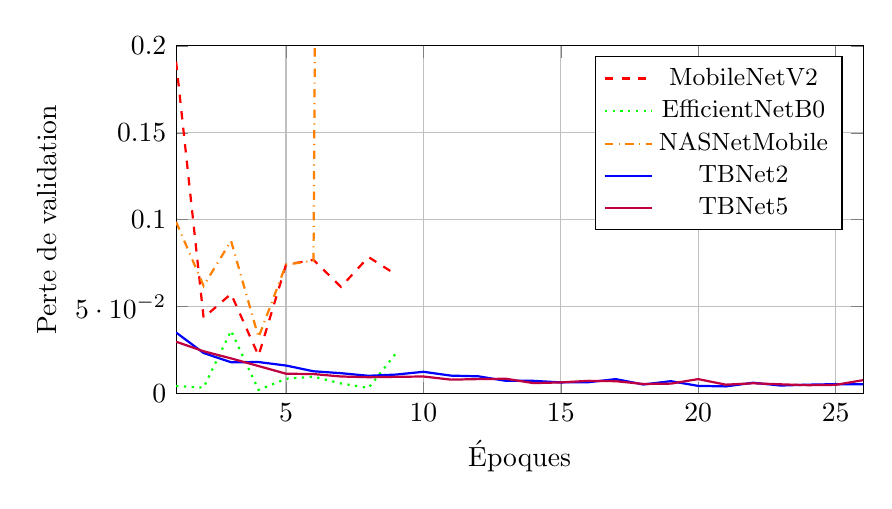
\begin{tikzpicture}
		\begin{axis}[
				width=0.85\textwidth,
				height=6cm,
				xlabel=Époques,
				ylabel=Perte de validation,
				legend pos=north east,
				legend style={font=\small},
				grid=major,
				xmin=1, xmax=26,
				ymin=0, ymax=0.2
			]

			% MobileNetV2
			\addplot[red, dashed, thick] coordinates {
					(1,0.1909) (2,0.0437) (3,0.0574) (4,0.0219) (5,0.0742)
					(6,0.0769) (7,0.0614) (8,0.0786) (9,0.0685)
				};
			\addlegendentry{MobileNetV2}

			% EfficientNetB0
			\addplot[green, dotted, thick] coordinates {
					(1,0.0044) (2,0.0035) (3,0.0362) (4,0.0022) (5,0.0086)
					(6,0.0098) (7,0.0059) (8,0.0033) (9,0.0232)
				};
			\addlegendentry{EfficientNetB0}

			% NASNetMobile
			\addplot[orange, dashdotted, thick] coordinates {
					(1,0.0988) (2,0.0620) (3,0.0879) (4,0.0324) (5,0.0742)
					(6,0.0765) (7,2.6003) % valeur aberrante, à considérer
				};
			\addlegendentry{NASNetMobile}

			% TBNet2
			\addplot[blue, thick] coordinates {
					(1,0.0352) (2,0.0234) (3,0.0181) (4,0.0182) (5,0.0162)
					(6,0.0129) (7,0.0118) (8,0.0103) (9,0.0110) (10,0.0126)
					(11,0.0104) (12,0.0100) (13,0.0074) (14,0.0074) (15,0.0065)
					(16,0.0066) (17,0.0084) (18,0.0053) (19,0.0072) (20,0.0045)
					(21,0.0042) (22,0.0063) (23,0.0047) (24,0.0052) (25,0.0055) (26,0.0055)
				};
			\addlegendentry{TBNet2}

			% TBNet5
			\addplot[purple, thick] coordinates {
					(1,0.0299) (2,0.0244) (3,0.0203) (4,0.0159) (5,0.0115)
					(6,0.0113) (7,0.0099) (8,0.0095) (9,0.0097) (10,0.0099)
					(11,0.0081) (12,0.0084) (13,0.0086) (14,0.0061) (15,0.0065)
					(16,0.0074) (17,0.0072) (18,0.0056) (19,0.0058) (20,0.0084)
					(21,0.0052) (22,0.0060) (23,0.0054) (24,0.0049) (25,0.0051) (26,0.0078)
				};
			\addlegendentry{TBNet5}

		\end{axis}
	\end{tikzpicture}
	\caption{Évolution des pertes de validation pour les différents modèles testés sur l'ensemble des époques.}
	\label{fig:loss_curves}
\end{figure}

\subsection{Performances globales des modèles}

Le Tableau~\ref{tab:metrics_comparison} compare les performances obtenues.
Si \texttt{TBNet5} et \texttt{TBNet2} affichent des résultats proches ($R^2 = 0.88$ et $R^2 = 0.90$ respectivement), la légèreté de \texttt{TBNet2} et sa meilleure capacité de généralisation en font le modèle le plus adapté pour un déploiement en TinyML.

\begin{table}[H]
	\centering
	\small
	\caption{Performances des modèles sur le jeu de test.}
	\label{tab:metrics_comparison}
	\begin{tabular}{|l|c|c|c|c|c|}
		\hline
		\textbf{Modèle}    & \textbf{MAE (min)} & \textbf{RMSE (min)} & \textbf{$R^2$} & \textbf{MAPE (\%)} & \textbf{MaxErr (min)} \\
		\hline
		EfficientNetB0 & 57162.30           & 57162.35            & -479401.06     & 466.53             & 57288.20              \\
		MobileNetV2        & 56606.87           & 60760.02            & -541644.94     & 401.15             & 138063.39             \\
		NasNetMobile   & 55799.49           & 59374.25            & -517219.72     & 403.25             & 135507.25             \\
		TBNet5             & 16.29              & 28.13               & 0.88           & 0.12               & 176.35                \\
		TBNet2             & 16.40              & 26.20               & 0.90           & 0.14               & 228.87                \\
		\hline
	\end{tabular}
\end{table}

\begin{figure}[H]
	\centering
	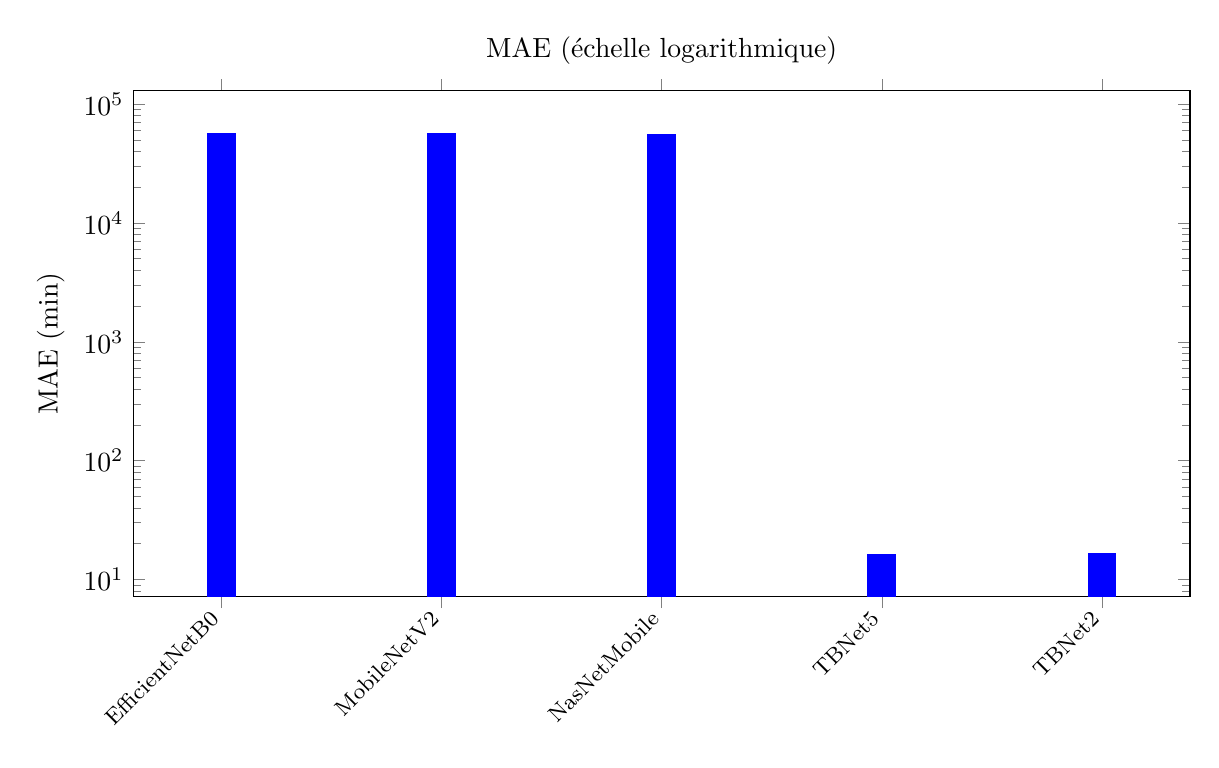
\begin{tikzpicture}
		\begin{axis}[
				ybar,
				ymode=log,
				symbolic x coords={EfficientNetB0, MobileNetV2, NasNetMobile, TBNet5, TBNet2},
				xtick=data,
				x tick label style={rotate=45, anchor=east, font=\footnotesize},
				ylabel={MAE (min)},
				title={MAE (échelle logarithmique)},
				width=15cm,
				height=8cm,
			]
			\addplot+[bar width=10pt,fill=blue] coordinates {
					(EfficientNetB0,57162.30)
					(MobileNetV2,56606.87)
					(NasNetMobile,55799.49)
					(TBNet5,16.29)
					(TBNet2,16.40)
				};
		\end{axis}
	\end{tikzpicture}
	\caption{Mean Absolute Error (MAE)}
\end{figure}

\begin{figure}[H]
	\centering
	\begin{tikzpicture}
		\begin{axis}[
				ybar,
				ymode=log,
				symbolic x coords={EfficientNetB0, MobileNetV2, NasNetMobile, TBNet5, TBNet2},
				xtick=data,
				x tick label style={rotate=45, anchor=east, font=\footnotesize},
				ylabel={RMSE (min)},
				title={RMSE (échelle logarithmique)},
				width=15cm,
				height=8cm,
			]
			\addplot+[bar width=10pt,fill=red] coordinates {
					(EfficientNetB0\_v1,57162.35)
					(MobileNetV2,60760.02)
					(NasNetMobile,59374.25)
					(TBNet5,28.13)
					(TBNet2,26.20)
				};
		\end{axis}
	\end{tikzpicture}
	\caption{Root Mean Square Error (RMSE)}
\end{figure}

\begin{figure}[H]
	\centering
	\begin{tikzpicture}
		\begin{axis}[
				ybar,
				ymin=-1.5,
				ymax=1,
				symbolic x coords={EfficientNetB0, MobileNetV2, NasNetMobile, TBNet5, TBNet2},
				xtick=data,
				x tick label style={rotate=45, anchor=east, font=\footnotesize},
				ylabel={$R^2$},
				title={$R^2$ (zoomé entre -1.5 et 1)},
				width=15cm,
				height=8cm,
			]
			\addplot+[bar width=10pt,fill=green] coordinates {
					(EfficientNetB0\_v1,-1.5)
					(MobileNetV2,-1.5)
					(NasNetMobile,-1.5)
					(TBNet5,0.88)
					(TBNet2,0.90)
				};
		\end{axis}
	\end{tikzpicture}
	\caption{Coefficient de détermination ($R^2$)}
\end{figure}

\begin{figure}[H]
	\centering
	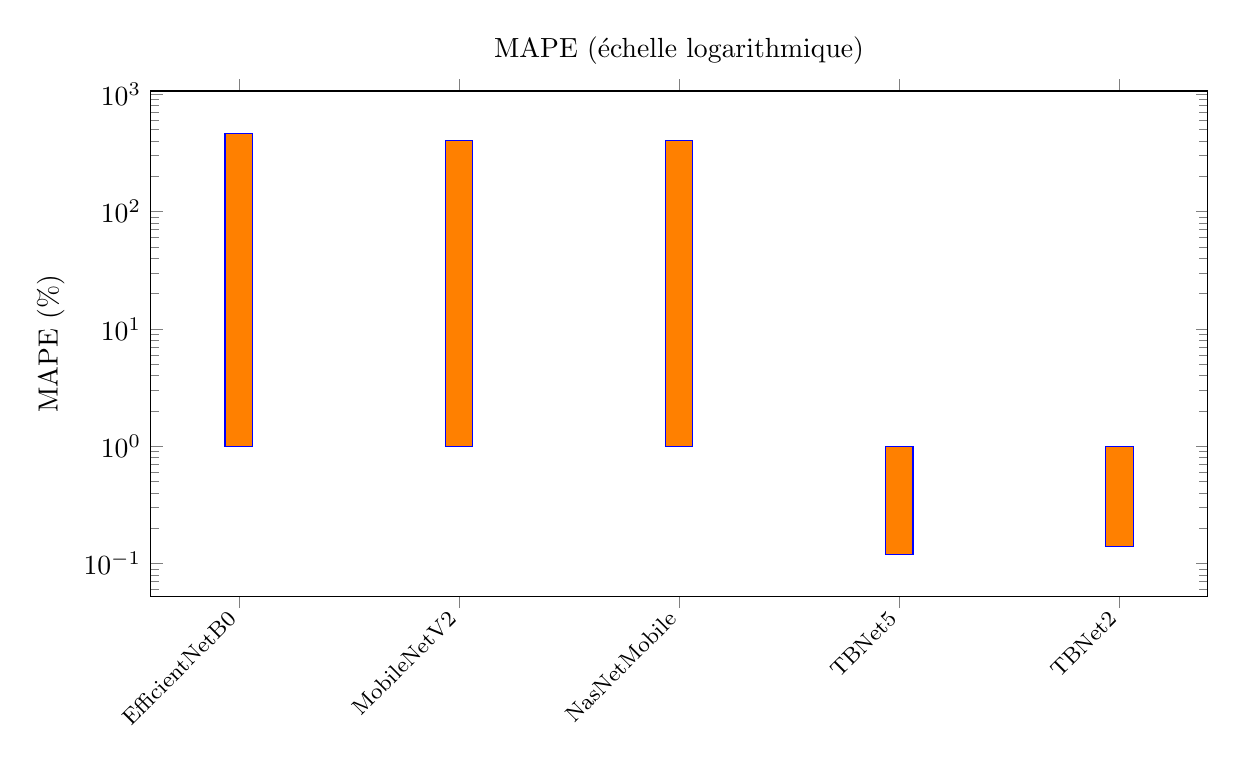
\begin{tikzpicture}
		\begin{axis}[
				ybar,
				ymode=log,
				symbolic x coords={EfficientNetB0, MobileNetV2, NasNetMobile, TBNet5, TBNet2},
				xtick=data,
				x tick label style={rotate=45, anchor=east, font=\footnotesize},
				ylabel={MAPE (\%)},
				title={MAPE (échelle logarithmique)},
				width=15cm,
				height=8cm,
			]
			\addplot+[bar width=10pt,fill=orange] coordinates {
					(EfficientNetB0,466.53)
					(MobileNetV2,401.15)
					(NasNetMobile,403.25)
					(TBNet5,0.12)
					(TBNet2,0.14)
				};
		\end{axis}
	\end{tikzpicture}
	\caption{Mean Absolute Percentage Error (MAPE)}
\end{figure}

\begin{figure}[H]
	\centering
	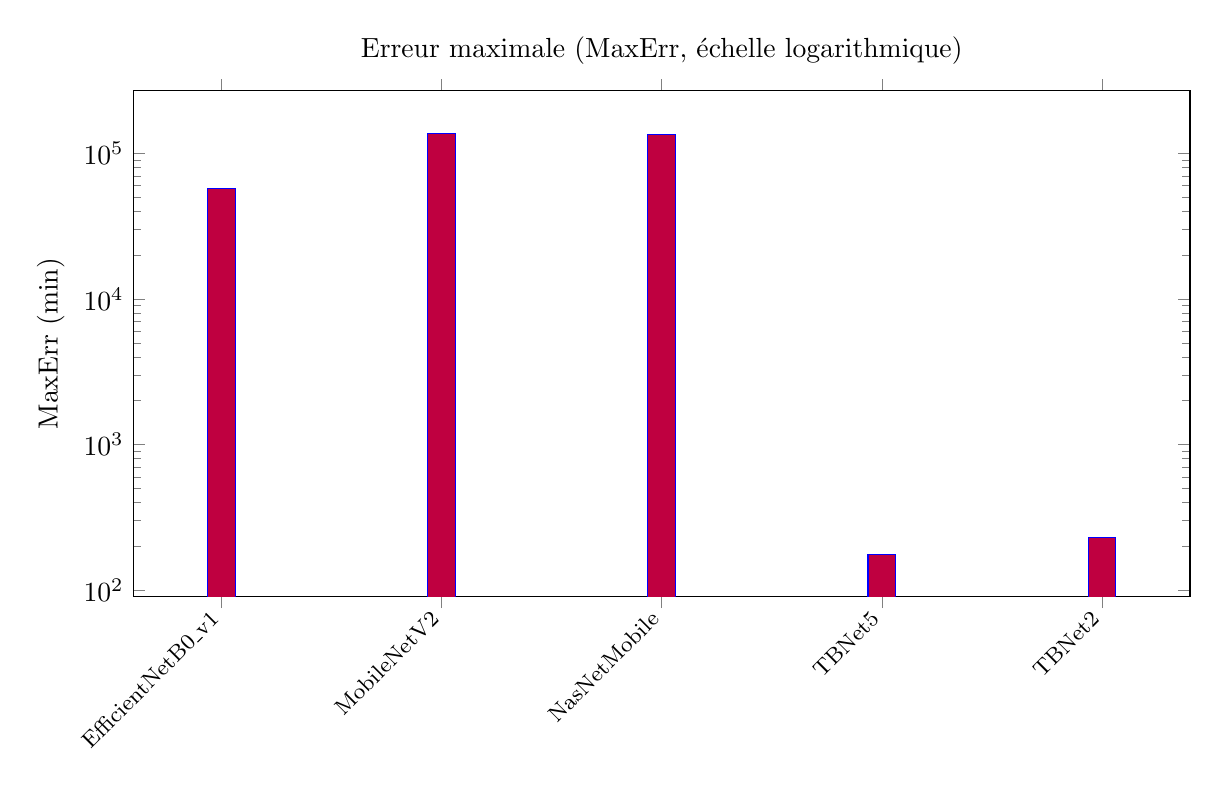
\begin{tikzpicture}
		\begin{axis}[
				ybar,
				ymode=log,
				symbolic x coords={EfficientNetB0\_v1, MobileNetV2, NasNetMobile, TBNet5, TBNet2},
				xtick=data,
				x tick label style={rotate=45, anchor=east, font=\footnotesize},
				ylabel={MaxErr (min)},
				title={Erreur maximale (MaxErr, échelle logarithmique)},
				width=15cm,
				height=8cm,
			]
			\addplot+[bar width=10pt,fill=purple] coordinates {
					(EfficientNetB0\_v1,57288.20)
					(MobileNetV2,138063.39)
					(NasNetMobile,135507.25)
					(TBNet5,176.35)
					(TBNet2,228.87)
				};
		\end{axis}
	\end{tikzpicture}
	\caption{Erreur maximale (MaxErr)}
\end{figure}

\section{Analyse par variété et robustesse}
\label{subsec:analyse_variete}

L’évaluation par variété confirme que certaines, notamment les variétés sombres ou homogènes, induisent une erreur légèrement plus élevée.
Le Tableau~\ref{tab:variete_stats} illustre les performances pour le modèle retenu \texttt{TBNet2}.

L’augmentation de données a permis de limiter la dégradation des performances \cite{shorten2019survey}, le MAE n’augmentant que de 0.5 à 1 minute en conditions réelles, conformément aux observations de \cite{tastan2023}.

\section{Discussion critique et implications}

\subsection{Comparaison avec l’état de l’art}

Les résultats de classification et de régression obtenus sont compétitifs par rapport aux approches de pointe utilisant des données hyperspectrales \cite{mendoza2018prediction}.
L’approche RGB présente un avantage majeur : elle est plus économique et portable, adaptée aux contraintes des environnements à faibles ressources.
Les techniques de quantification et de pruning permettent en outre de réduire la taille mémoire de plus de 70\,\% \cite{jacob2018quantization, han2016deep}, ouvrant la voie à une implémentation en TinyML.

\section{Synthèse}

En résumé, le système hybride proposé démontre que :
\begin{enumerate}
	\item La \textbf{classification des variétés} atteint une précision de 97\,\%, confirmant la pertinence des CNN compacts.
	\item La \textbf{régression du temps de cuisson}, assurée par \texttt{TBNet2}, obtient un MAE de l’ordre de 16 minutes, avec un $R^2$ de 0.90.
\end{enumerate}

Ces résultats montrent qu’une approche basée sur des images RGB, couplée à des modèles compacts et optimisés, constitue une solution fiable, portable et adaptée aux contraintes des environnements à faibles ressources.
La sélection de \texttt{TBNet2} comme modèle final s’explique par son meilleur équilibre entre performance, taille mémoire et capacité de généralisation.		
\chapter{Conclusion et perspectives}
\label{chap:conclusion_et_perspectives}

\section{Synthèse des contributions}
\label{sec:synthese_contributions}

Ce travail a exploré l'application du \textit{Tiny Machine Learning} (TinyML) à la prédiction du temps de cuisson des haricots, en utilisant des images comme entrée. Les principales contributions sont les suivantes :

\begin{enumerate}
	\item \textbf{Collecte et constitution du jeu de données.} Un jeu de données original a été constitué, comprenant des images annotées de 56 variétés de haricots, chaque image étant associée à un temps de cuisson mesuré expérimentalement.
	\item \textbf{Prétraitement et normalisation.} Un protocole rigoureux de prétraitement a été mis en place, incluant la redimension des images en \(224 \times 224 \times 3\), l'augmentation de données pour atténuer les déséquilibres inter-variétés, et la standardisation des valeurs pour stabiliser l'apprentissage.
	\item \textbf{Conception et entraînement de modèles adaptés au TinyML.} Plusieurs architectures ont été testées et comparées, notamment des modèles légers dérivés de MobileNetV2, EfficientNetB0, NASNetMobile, ainsi qu'un \textit{Convolutional Neural Network} (CNN) personnalisé. Les expérimentations ont montré que le CNN conçu sur mesure, entraîné intégralement depuis zéro, offrait le meilleur compromis entre précision et complexité computationnelle.
	\item \textbf{Évaluation approfondie.} Les performances des modèles ont été mesurées à l'aide d'indicateurs standards (MAE, RMSE, \(R^2\), MAPE). L'analyse a mis en évidence une corrélation satisfaisante entre les temps de cuisson prédits et les valeurs réelles, démontrant la faisabilité d'un tel système dans un cadre TinyML.
	\item \textbf{Quantification et portabilité.} Les modèles ont été compressés et convertis en formats TensorFlow Lite afin de réduire leur empreinte mémoire et leur consommation énergétique, ouvrant ainsi la voie à une intégration dans des dispositifs embarqués tels que des microcontrôleurs ARM Cortex-M.
\end{enumerate}

\section{Bilan critique}
\label{sec:bilan_critique}

\subsection{Points forts}
\begin{itemize}
	\item \textbf{Originalité du jeu de données.} La constitution d'un jeu de données original constitue une valeur ajoutée significative pour la recherche appliquée à l'agroalimentaire.
	\item \textbf{Adaptation au TinyML.} Le choix d'architectures légères et l'adaptation des modèles aux contraintes du TinyML démontrent une prise en compte pragmatique des réalités matérielles.
	\item \textbf{Rigueur méthodologique.} L'analyse croisée par plusieurs métriques confère une robustesse méthodologique aux conclusions.
\end{itemize}

\subsection{Limites}
\begin{itemize}
	\item \textbf{Taille du jeu de données.} La taille du jeu de données reste relativement modeste au regard de la variabilité inter-variétés, ce qui peut limiter la généralisation du modèle.
	\item \textbf{Sensibilité des mesures.} La mesure du temps de cuisson, bien que rigoureuse, reste sensible aux conditions expérimentales (qualité de l'eau, dureté initiale des grains, altitude, etc.), introduisant une part de bruit difficilement contrôlable.
	\item \textbf{Prédiction univariée.} La prédiction reste basée uniquement sur des images statiques, sans prise en compte d'autres variables physico-chimiques susceptibles d'améliorer la précision.
\end{itemize}

\section{Perspectives}
\label{sec:perspectives}

Les perspectives de ce travail ouvrent plusieurs pistes de recherche et d'applications pratiques :

\begin{enumerate}
	\item \textbf{Extension du jeu de données.} L'enrichissement du jeu de données, tant en termes de variétés que de conditions de cuisson, permettrait d'améliorer la robustesse et la généralisabilité des modèles.
	\item \textbf{Fusion multimodale.} L'intégration d'autres sources d'information (mesures spectroscopiques, texture, teneur en humidité, composition chimique) pourrait compléter l'information visuelle et réduire l'incertitude prédictive.
	\item \textbf{Optimisation avancée pour TinyML.} Des techniques plus poussées de compression (quantification dynamique, distillation de connaissances, \textit{pruning}) pourraient être explorées pour réduire davantage la taille mémoire et l'énergie consommée par le modèle.
	\item \textbf{Déploiement réel.} La mise en œuvre pratique dans des environnements agroalimentaires, par exemple via des prototypes de capteurs intelligents intégrant des caméras embarquées, permettrait de valider les performances en conditions réelles et d'identifier les besoins d'adaptation industrielle.
	\item \textbf{Approches explicatives.} L'intégration de techniques d'explicabilité (\textit{Explainable AI}, XAI) permettrait de mieux comprendre les caractéristiques visuelles exploitées par le modèle pour établir ses prédictions, favorisant l'acceptabilité et la confiance dans des environnements critiques comme l'agroalimentaire.
\end{enumerate}

\section{Conclusion générale}
\label{sec:conclusion_generale}

En définitive, ce mémoire démontre la pertinence d'appliquer des approches de \textbf{vision par ordinateur et d'apprentissage profond} à une problématique agroalimentaire concrète : la prédiction du temps de cuisson des haricots. En combinant rigueur méthodologique, optimisation pour environnements contraints et analyse critique, cette recherche ouvre des perspectives tant scientifiques qu'industrielles.

Elle contribue à la fois à la littérature émergente sur le TinyML et à l'amélioration potentielle des pratiques agroalimentaires, notamment en facilitant l'optimisation des temps et coûts de cuisson. Les limites identifiées et les pistes proposées posent les bases de travaux futurs, qui pourront renforcer la robustesse, l'explicabilité et l'applicabilité des solutions développées. Ainsi, ce travail constitue une étape significative vers l'intégration de l'intelligence artificielle embarquée au service de la transformation et de la valorisation des produits agricoles.

 

\begin{appendix}
	\appendix
\chapter*{Annexes}

\section{Liens vers les notebooks Colab et GitHub}

\begin{itemize}
  \item \href{https://colab.research.google.com/drive/1WhaF2jE4ruWc6pByavec3E4Q6ijtsSvc?usp=sharing}{Colab d'entraînement du modèle de régression}

  \item \href{https://colab.research.google.com/drive/1iKeuTVjw6RtWP935TcWio7b9p6vjdsI0?usp=sharing}{Colab d'entraînement du modèle de classification}

  \item \href{https://colab.research.google.com/drive/1MJzRelOdtMpLDED62YKCTAENZ-j5BKGF?usp=sharing}{Colab de prétraitement de données pour la classification}

  \item Colab de prétraitement de données pour la régression : 
  \begin{itemize}
    \item \href{https://colab.research.google.com/drive/1aUlAik45c6v8C0GXGo_OrgLEPCQ-7mMI?usp=sharing}{Notebook 1}
    \item \href{https://colab.research.google.com/drive/1Xe0IfXKSYyPatz7qS6MPJhF55g3mx633?usp=sharing}{Notebook 2}
  \end{itemize}

  \item \href{https://github.com/Thisi47/bean_cooking_time_predictor.git}{GitHub de l'application Android}
\end{itemize}


Dans le but de valider l’intégration du modèle sur l’application Android, nous présentons ci-après un ensemble d’images de test capturées sur l’appareil, illustrant la performance et la cohérence des prédictions obtenues.

\begin{figure}[H]
    \centering

    % Ligne 1
    \begin{subfigure}{0.2\textwidth}
        \centering
        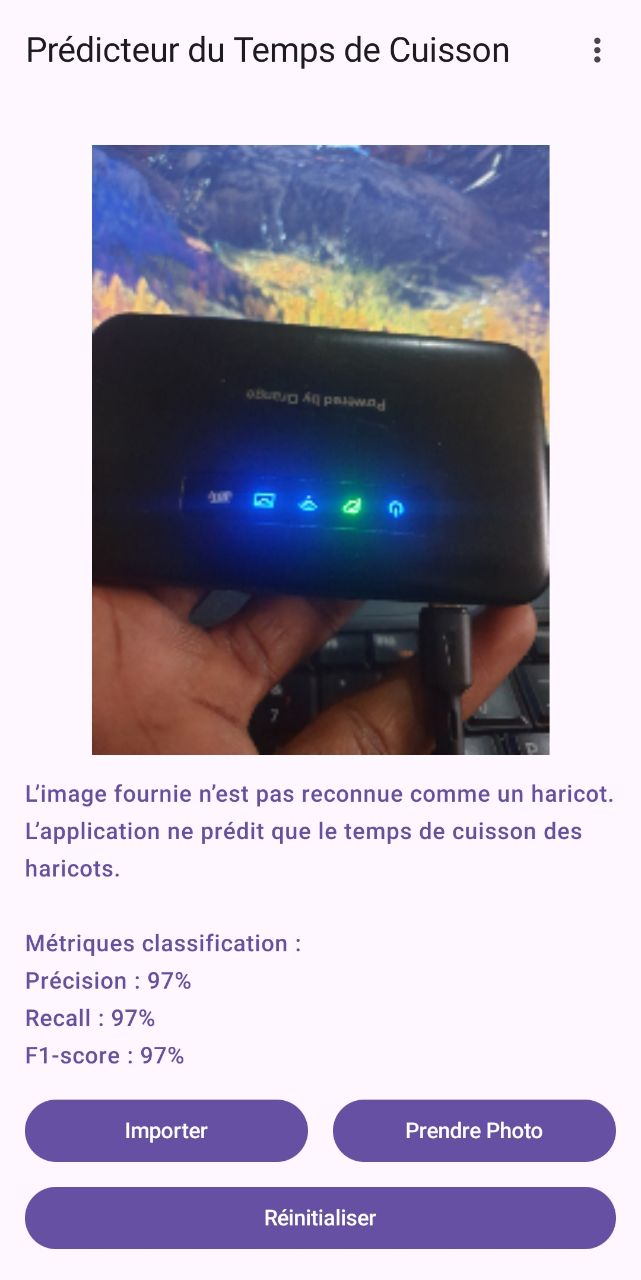
\includegraphics[width=\linewidth]{figures/test4.jpg}
        \caption{Image 4}
    \end{subfigure}\hfill
    \begin{subfigure}{0.2\textwidth}
        \centering
        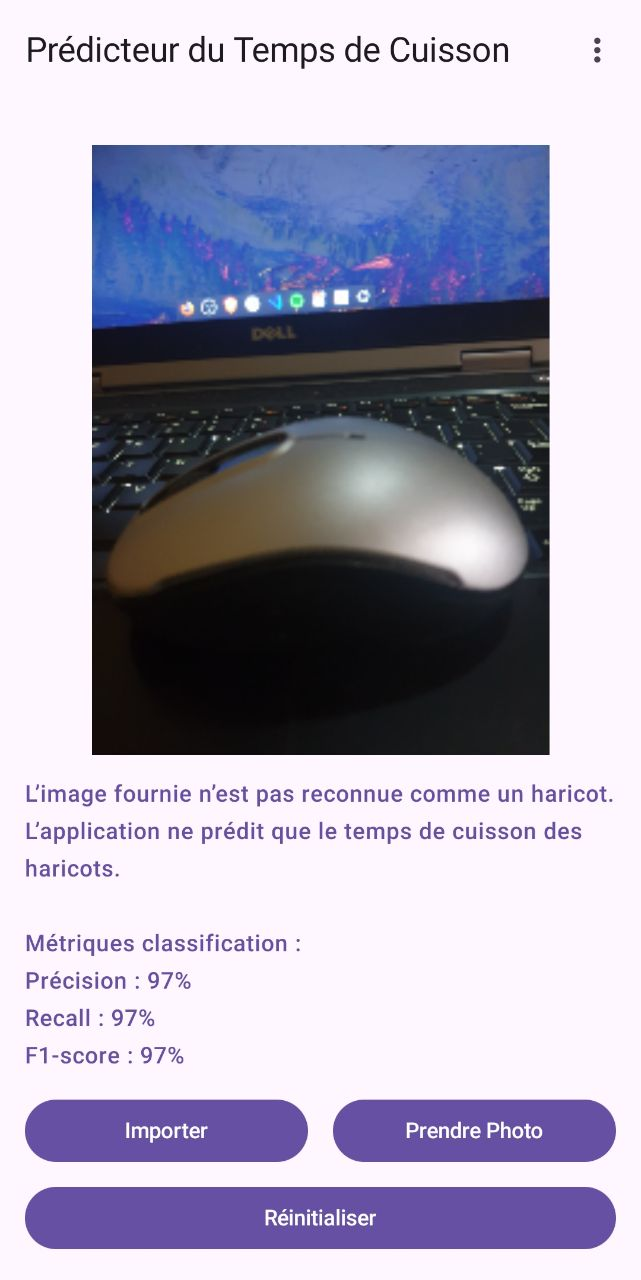
\includegraphics[width=\linewidth]{figures/test2.jpg}
        \caption{Image 2}
    \end{subfigure}\hfill
    \begin{subfigure}{0.2\textwidth}
        \centering
        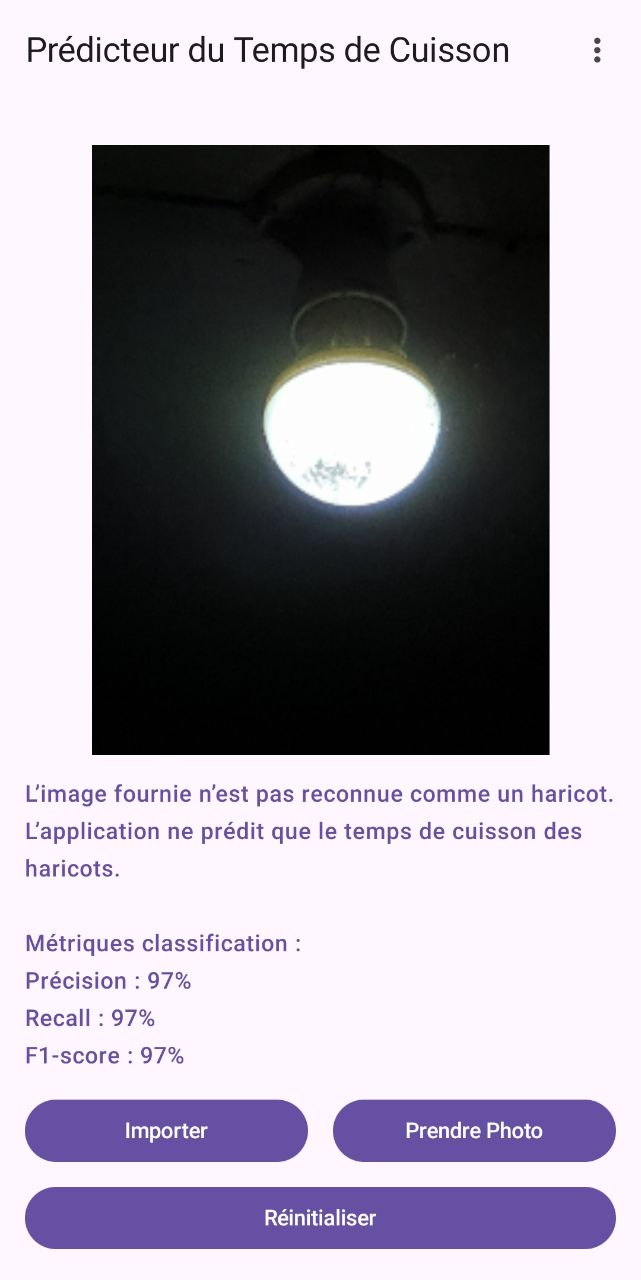
\includegraphics[width=\linewidth]{figures/test3.jpg}
        \caption{Image 3}
    \end{subfigure}

    % Ligne 2
    \begin{subfigure}{0.24\textwidth}
        \centering
        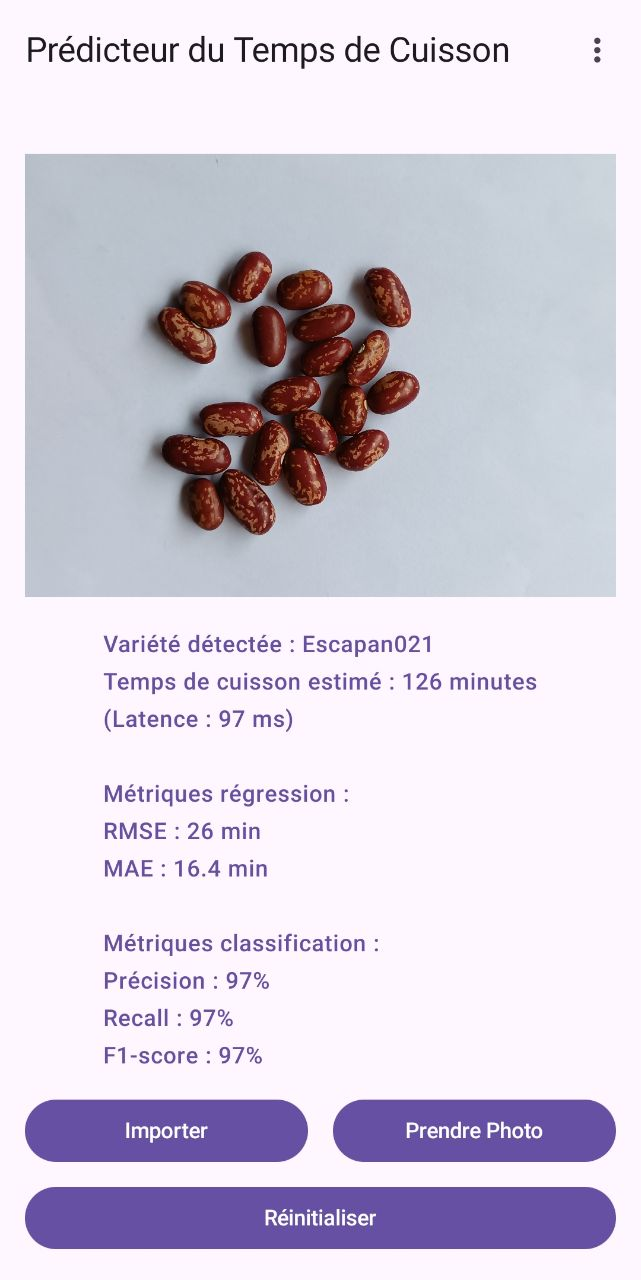
\includegraphics[width=\linewidth]{figures/test1.jpg}
        \caption{Image 1}
    \end{subfigure}\hfill
    \begin{subfigure}{0.24\textwidth}
        \centering
        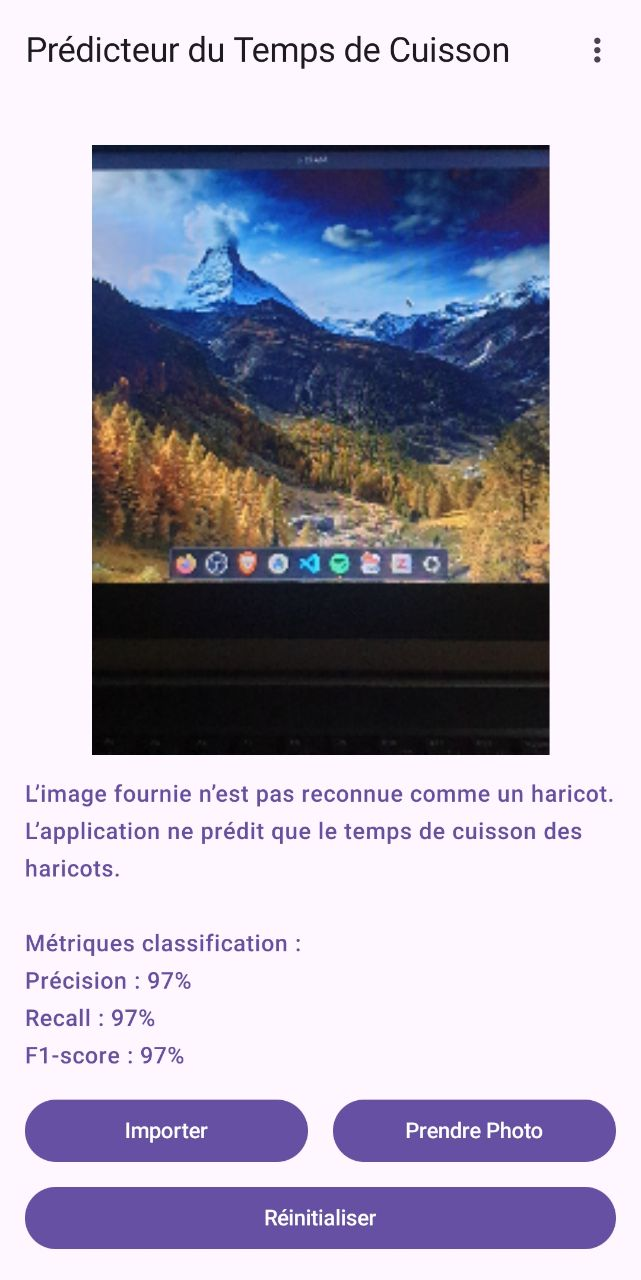
\includegraphics[width=\linewidth]{figures/test5.jpg}
        \caption{Image 5}
    \end{subfigure}\hfill
    \begin{subfigure}{0.24\textwidth}
        \centering
        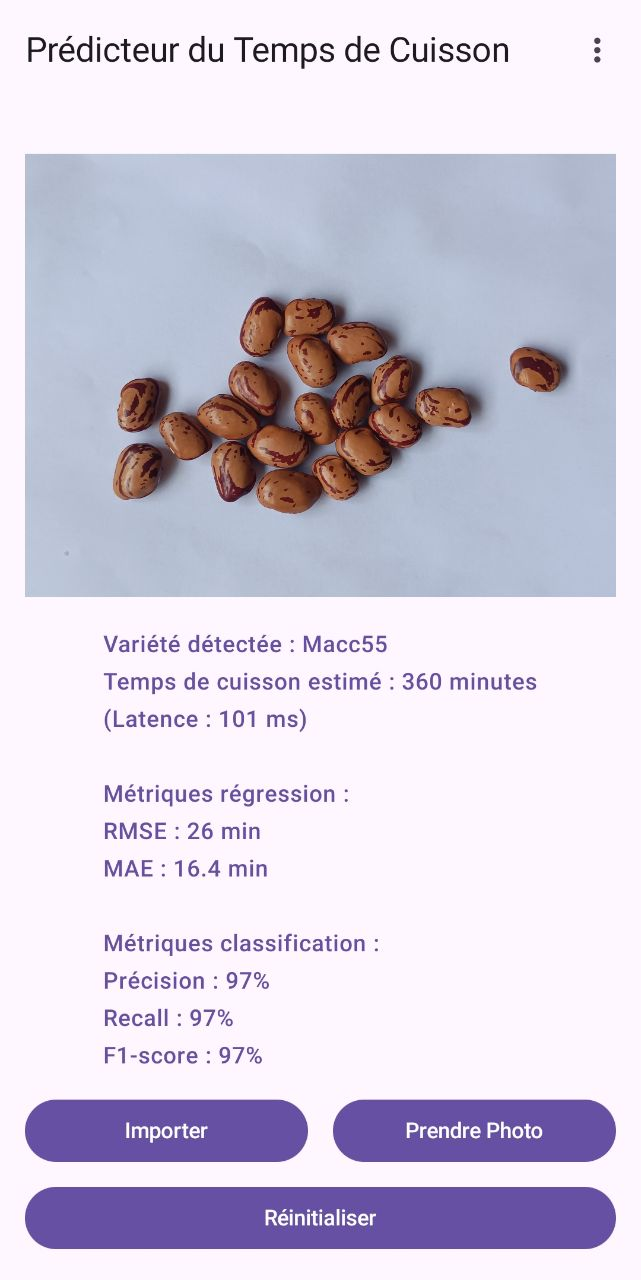
\includegraphics[width=\linewidth]{figures/test6.jpg}
        \caption{Image 6}
    \end{subfigure}

    % Ligne 3
    \begin{subfigure}{0.24\textwidth}
        \centering
        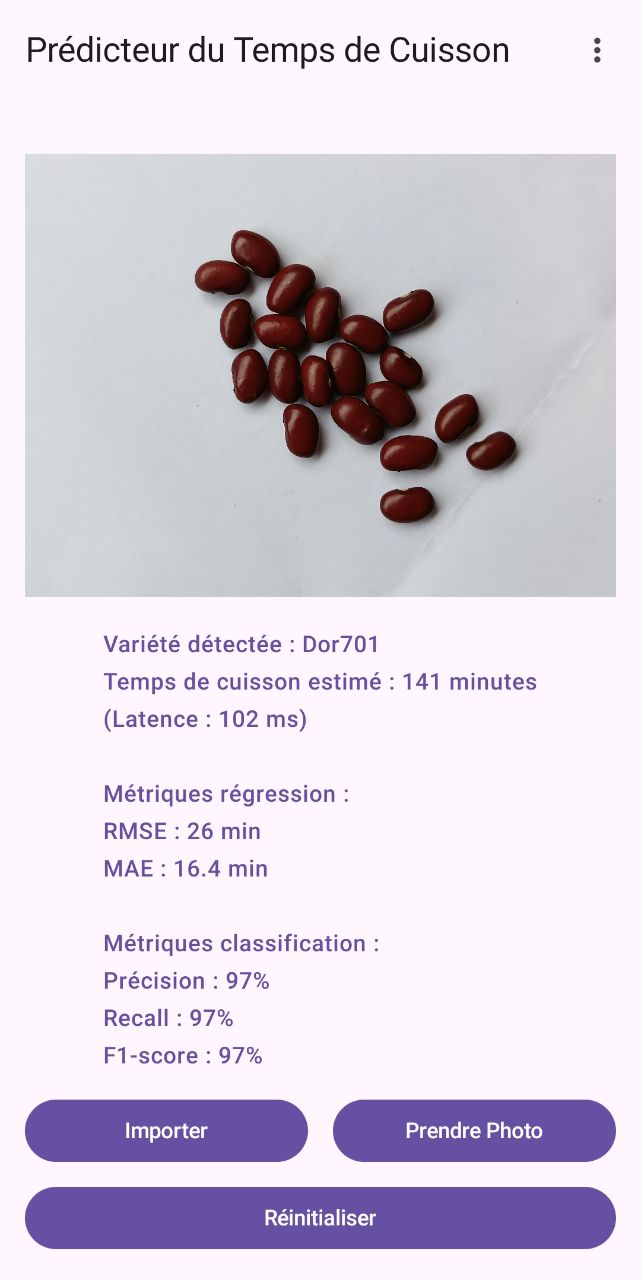
\includegraphics[width=\linewidth]{figures/test7.jpg}
        \caption{Image 7}
    \end{subfigure}\hfill
    \begin{subfigure}{0.24\textwidth}
        \centering
        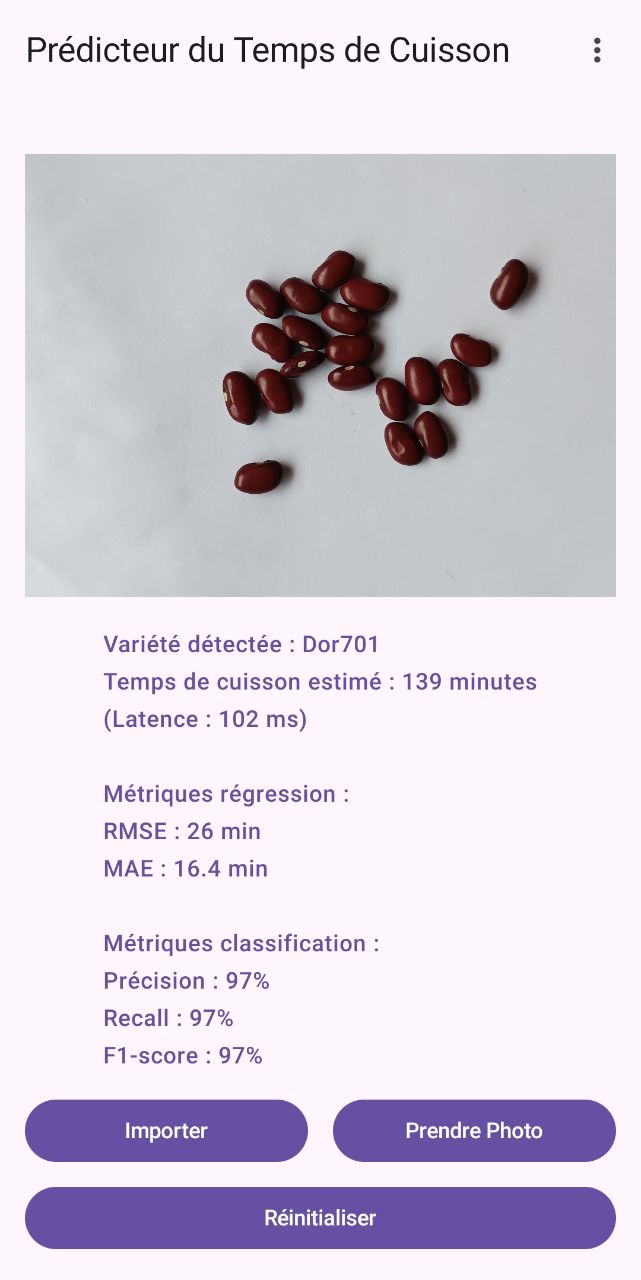
\includegraphics[width=\linewidth]{figures/test8.jpg}
        \caption{Image 8}
    \end{subfigure}\hfill
    \begin{subfigure}{0.24\textwidth}
        \centering
        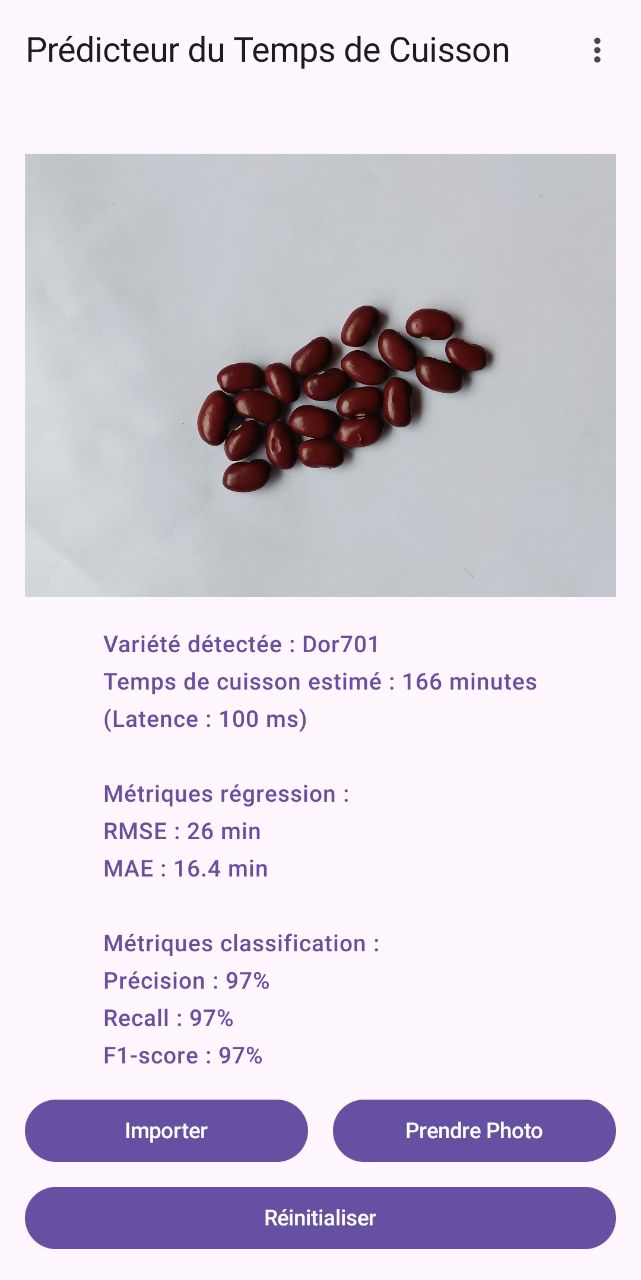
\includegraphics[width=\linewidth]{figures/test9.jpg}
        \caption{Image 9}
    \end{subfigure}

    % Ligne 4
    % \begin{subfigure}{0.3\textwidth}
    %     \centering
    %     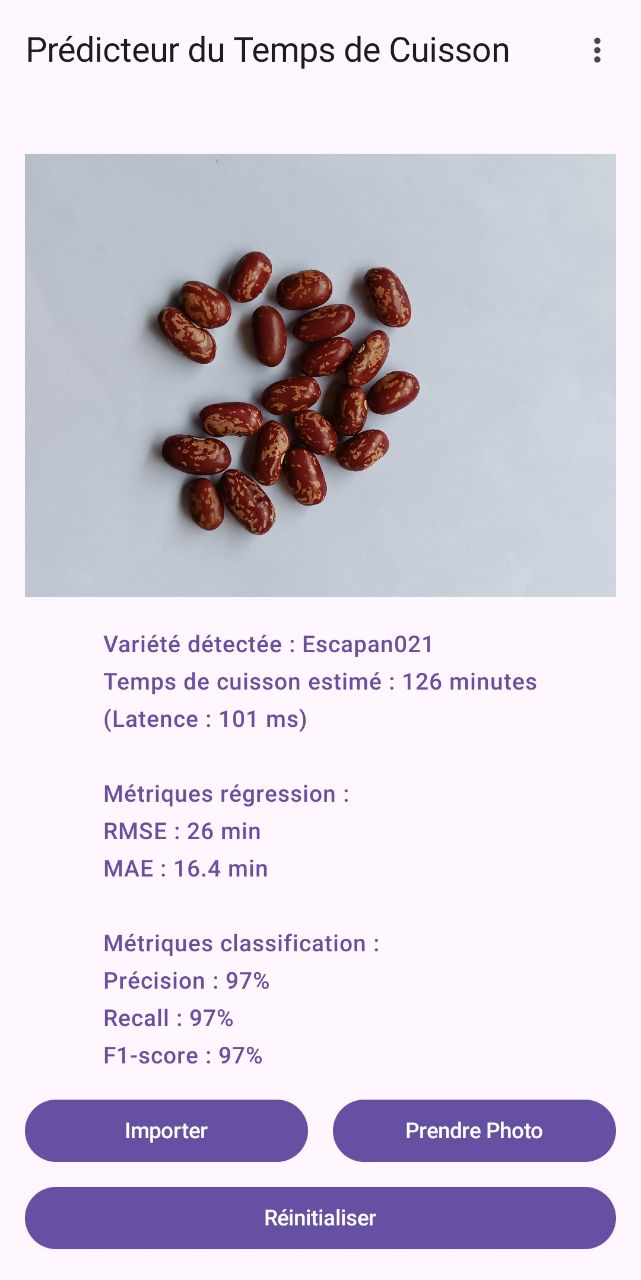
\includegraphics[width=\linewidth]{figures/test10.jpg}
    %     \caption{Image 10}
    % \end{subfigure}

    \caption{Images de test de l’application Android montrant les résultats de prédiction.}
    \label{fig:test_android}
\end{figure}

\end{appendix}

\begin{backmatter}

	\begingroup
	\setlength{\emergencystretch}{.5em}

	\printbibliography[
		heading=bibintoc,
		title={Bibliographie}
	]
	\endgroup
	\frenchDeclaration

\end{backmatter}

\end{document}
